\section{Results and discussions}\label{Section4}
For simplicity, the present work adopts a two-dimensional plane stress model. A rectangular plate with a pre-existing edge crack serves as an example, with its dimensions and boundary conditions shown in Figure \ref{fig1}(a). The pre-existing crack is defined by the local historical variable $H$, which is expressed in Eq.\eqref{historical variable}. Dimensionless parameters are utilized to ensure computational accuracy \cite{chang_liu_isogeometric_2019}. The top edge of the plate is subjected to a time-dependent displacement load, $u_y^*=0. 002\times t^*$ is applied for the quasi-static model, where $t^*$ represents time, and the asterisk (*) denotes a dimensionless quantity. The simulation of an applied external electric field is achieved by establishing varying electric potentials across specific boundaries.  Unless specifically stated, it is assumed that both mechanical and electrical boundary conditions are traction-free and electrically open-circuited. The model uses a discretization of $50 \times 50$ elements, with local refinement at the crack region, as illustrated in Figure \ref{fig1}(b).  The material chosen for analysis is single-crystal \ce{PbTiO3} with its parameters listed in Table \ref{table1}. 
 
\begin{figure}[htbp!]
    \centering
    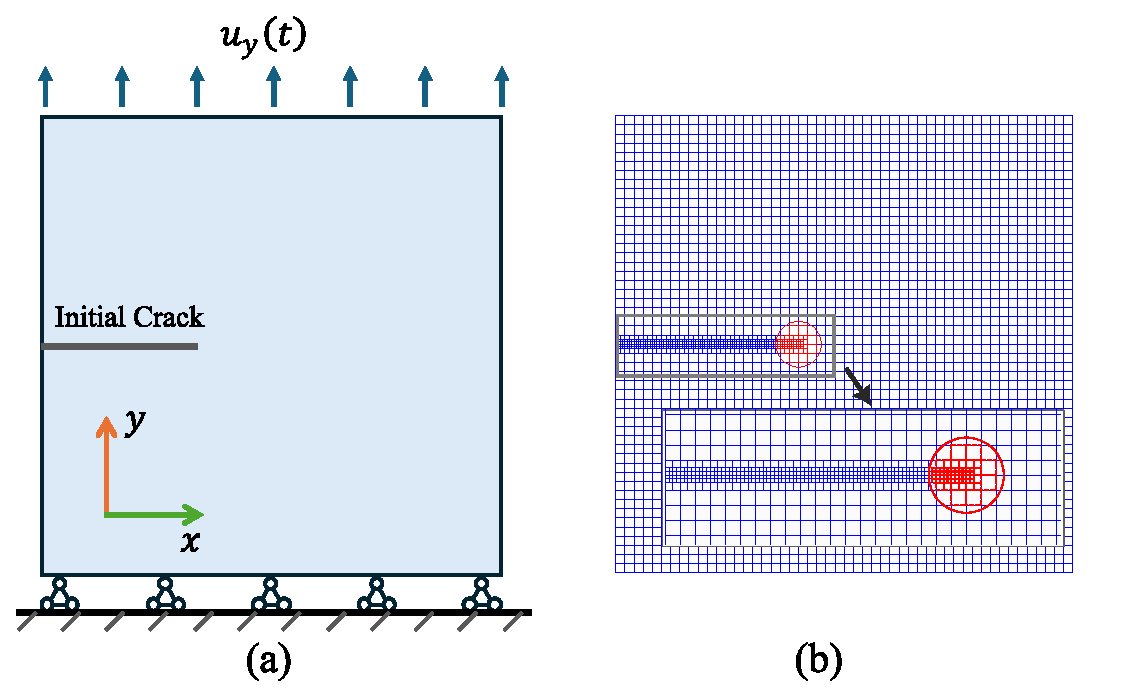
\includegraphics[width=\linewidth]{Fig1.eps}
    \caption{(a) Two-dimensional rectangular plate model and its corresponding boundary conditions. The dimension of the plate is 100 nm $\times$ 100 nm with a 40 nm pre-existing crack initiating from the left edge. Displacement along the $x_2$-axis is fixed at the bottom surface, while a time-dependent displacement, $u_2 (t)$, is imposed on the top surface. The origin of the coordinate system is located in the bottom left corner of the model. (b)  Mesh detail for the model. The discretized mesh is $50\times50$, with local refinement in the pre-existing crack area. The area enclosed by the gray box is an enlarged view of the local mesh around the crack. The regions marked by red circles and elements denote the area employed for calculating the configurational force.}
    \label{fig1}
\end{figure}

This section will primarily investigate two types of models: 1. The crack propagation direction is parallel to the polarization direction. This includes cases where both the crack and polarization directions align along the $x_1$-axis, and the case where the crack direction is opposite to the polarization direction (with polarization opposing the $x_1$-axis). 2. The crack propagation direction is perpendicular to the polarization direction, including cases with the polarization along the $x_2$-axis and cases with  polarization opposing the $x_2$-axs. In each case, domain evolution is initiated through a Gaussian random distribution of polarization. Before fracture evolution, polarization experiences enough time to relax sufficiently and form a stable domain structure. An impermeable crack boundary is employed to mimic air-filled cracks \cite{wang_effect_2010}. 

\begin{table}[!htbp]
    \centering
    \caption{Values of the dimensionless coefficients for \ce{PbTiO3}\cite{yong_zhang_phase_2022,eliseev_defect-driven_2018}}
    \label{table1}
    \begin{tabular}{lclcll}
        \toprule
        \multicolumn{6}{c}{Landau coeff.}                                                   \\ \midrule
        $\alpha_1$ & $\alpha_{11}$ & $\alpha_{12}$ & $\alpha_{111}$   & $\alpha_{112}$  &   \\
        -1.0          & -0.24            & 2.53             & 0.49               & 1.2               &   \\
        \multicolumn{3}{c}{gradient coeff.}        & \multicolumn{2}{c}{kinetic coeff.} &   \\ \cmidrule(r){1-3}\cmidrule(l){4-5}
        $G_{11}$   & $G_{12}$      & $G_{44}$      & $L_P$            & $L_\nu$         &   \\
        1.6          & 0             & 0.8             & 1.0                & 0.001               &   \\
        \multicolumn{2}{c}{elastic coeff.}        & \multicolumn{2}{c}{electrostrictive coeff.}      & \multicolumn{2}{c}{flexoelectric coeff.} \\ \cmidrule(r){1-2}\cmidrule{3-4}\cmidrule(l){5-6}
        $c_{11}$   & 1766             & $Q_{11}$      & 0.05                & $f_{11}$        & 51.7 \\
        $c_{12}$   & 802              & $Q_{12}$      &  -0.015              & $f_{12}$        & 37.3 \\
        $c_{44}$   & 1124             & $Q_{44}$      &  0.038              & $f_{44}$        & 42.6 \\
        \multicolumn{2}{c}{relative permittivity} & \multicolumn{2}{c}{critical energy release rate} & \multicolumn{2}{c}{length parameter}      \\ \cmidrule(r){1-2}\cmidrule{3-4}\cmidrule(l){5-6}
        $\kappa$   & 66            & $G_c$         & 20.2               & $l_0$           & 1 \\ \bottomrule
        \end{tabular}
\end{table}

\subsection{Crack parallel to the initial polarization direction}
To establish a single domain state with polarization vectors aligned along the $x_1$-axis, an external electric field $E_{1}^*=1$ is applied. This is achieved by setting the electric potential at the left and right edges to 0 and 100, respectively. 

\begin{figure}[!htbp]
    \centering
    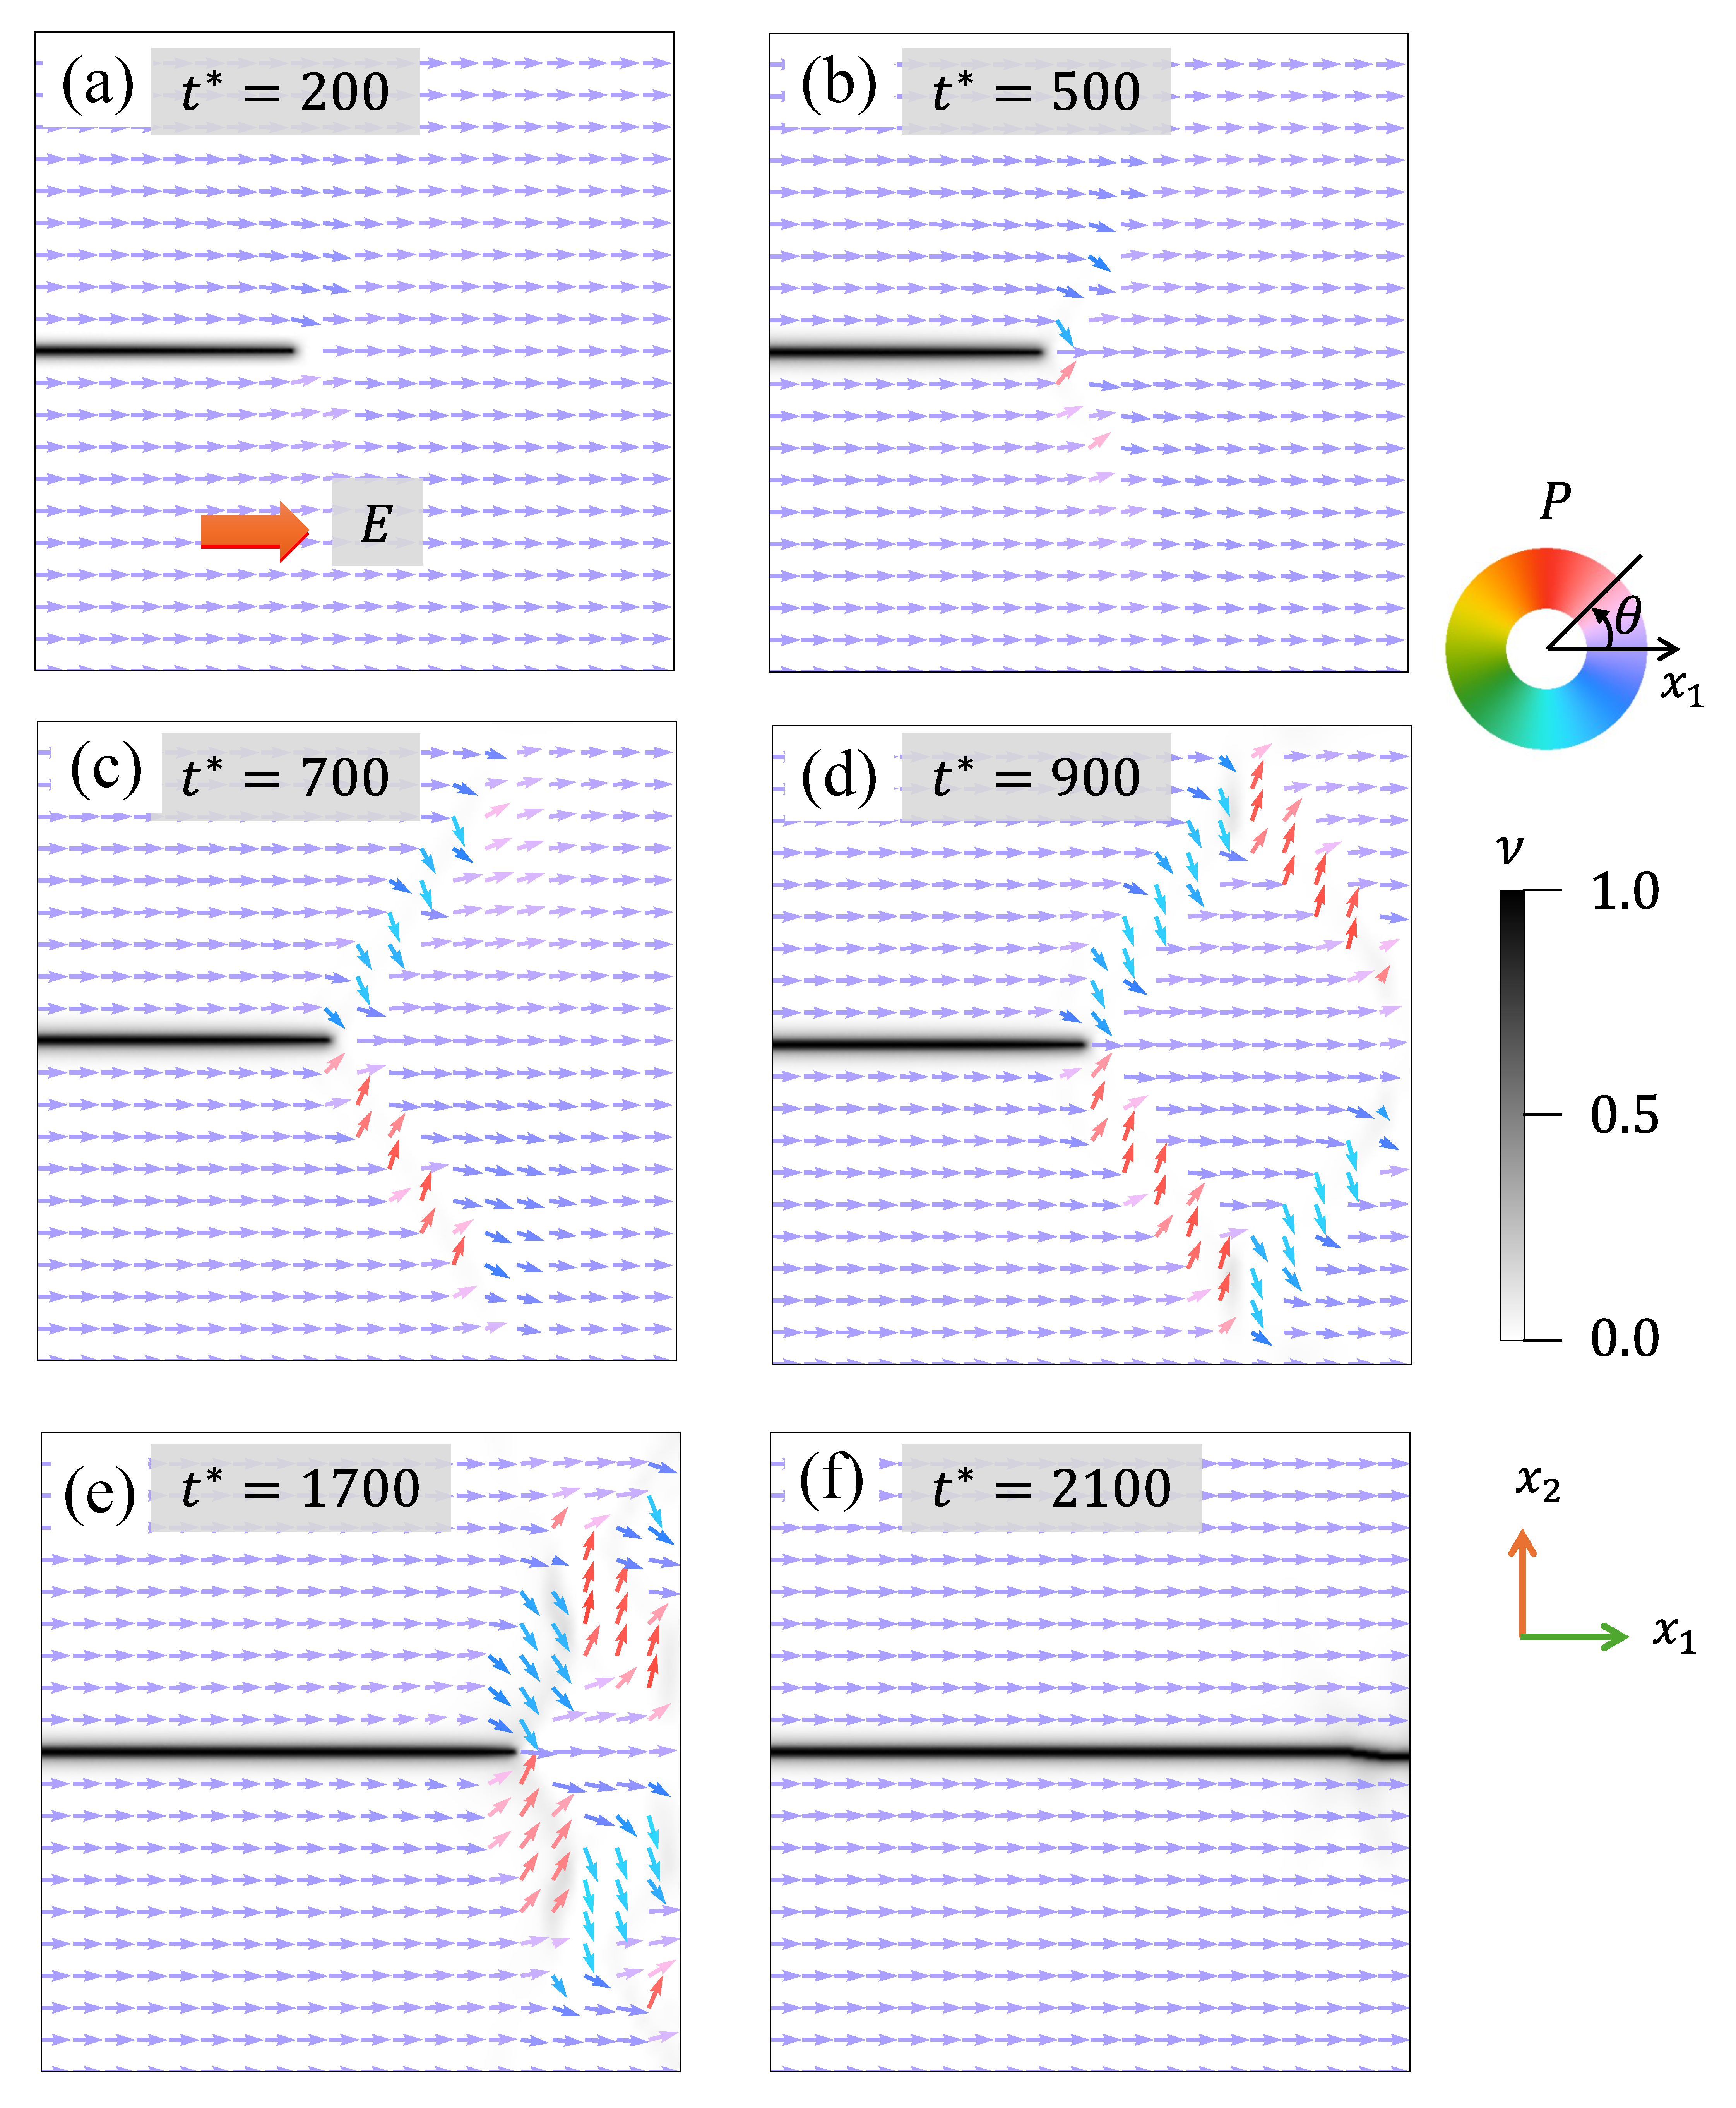
\includegraphics[width=\linewidth]{Fig2.pdf}
    \caption{Dynamic progressions of crack propagation and polarization switching across various time intervals. The grayscale maps illustrate the spatial distribution of the fracture order parameter $\nu$. The arrows indicate the orientation and magnitude of the polarization vectors, with the colors representing the angle of polarization relative to the $x_1$-axis.} \label{fig2}
\end{figure} 

Figure \ref{fig2} presents the temporal progression of the domain structure alongside crack propagation without flexoelectric effect ($f_{ij}=0$). Before crack propagation, the material maintains almost a single domain state. In the vicinity of the crack tip, some spontaneous polarization rotate by angles less than $45^\circ$, yet no distinct switched zone forms, as illustrated in Figure \ref{fig2}(a). As the load $u_2^*$ increases, the pre-existing crack begins to extend. A distinctly switched zone develops in front of the crack tip, which is distinguished by two forward wings. The shape of the switched zone is almost symmetric with respect to the crack, while the directions of polarization switching within it are notably asymmetric. Specifically, the polarization in the wing above the crack rotates $90^\circ$ clockwise, whereas those below the crack rotate $90^\circ$ counterclockwise. The magnitude of $u_2^*$ directly influences both the width and length of the switched zone, with a larger value of $u_2^*$ leading to a more expansive region, as demonstrated in Figures \ref{fig2}(b)-(c). Similar domain evolution process near the crack tip are also reported by Wang et al. \cite{wang_phase_2008}.  

As $u_2^*$ continues to increase, the crack further propagates, and the switched zone expands correspondingly. Once the foremost area of the switched zone reaches the edge of the plate, a reflection-like phenomenon occurs, causing the zone to expand forward at the same reflection angle, and the angle of polarization rotation changes symmetrically. In the newly formed switched zone above the crack, the polarization rotates $90^\circ$ clockwise, whereas the polarization below the crack rotates $90^\circ$ counterclockwise. At this stage, the overall domain structure within the plate still exhibits symmetry along the crack plane. Among the four switched zones, the polarization alternately aligns in the up and down directions, forming a diamond structure that encloses the unswitched region, as illustrated in Figure \ref{fig2}(d). With further increases in $u_2^*$, the envelope area of the switched zone gradually decreases, while the width of the switch zones slightly expands. Symmetrically, $90^\circ$ polarization switched zones also emerge in the upper right and lower right corners of the plate, as presented in Figure \ref{fig2}(e). Subsequently, as the load continues to increase, the crack propagates to the right boundary of the plate, resulting in a complete fracture. At this point, the two sections of the plate along the crack plane can be considered as two independent plates. The displacement load no longer affects the distribution of the domain structure, which is now entirely controlled by the electric field, leading to the formation of two single-domain regions oriented along the $x_1$-direction, as shown in Figure \ref{fig2}(f). Throughout the loading process, polarization switching maintains symmetry relative to the crack plane, and the crack propagation path remains a straight path. It is only at moments close to complete fracture that minor differences in the domain structures on either side of the crack amplify, leading to a deviation in the crack propagation path. The complete spatial and temporal evolution of the domain structure and crack path is presented in Video S1.

\begin{figure}[!htbp]
    \centering
    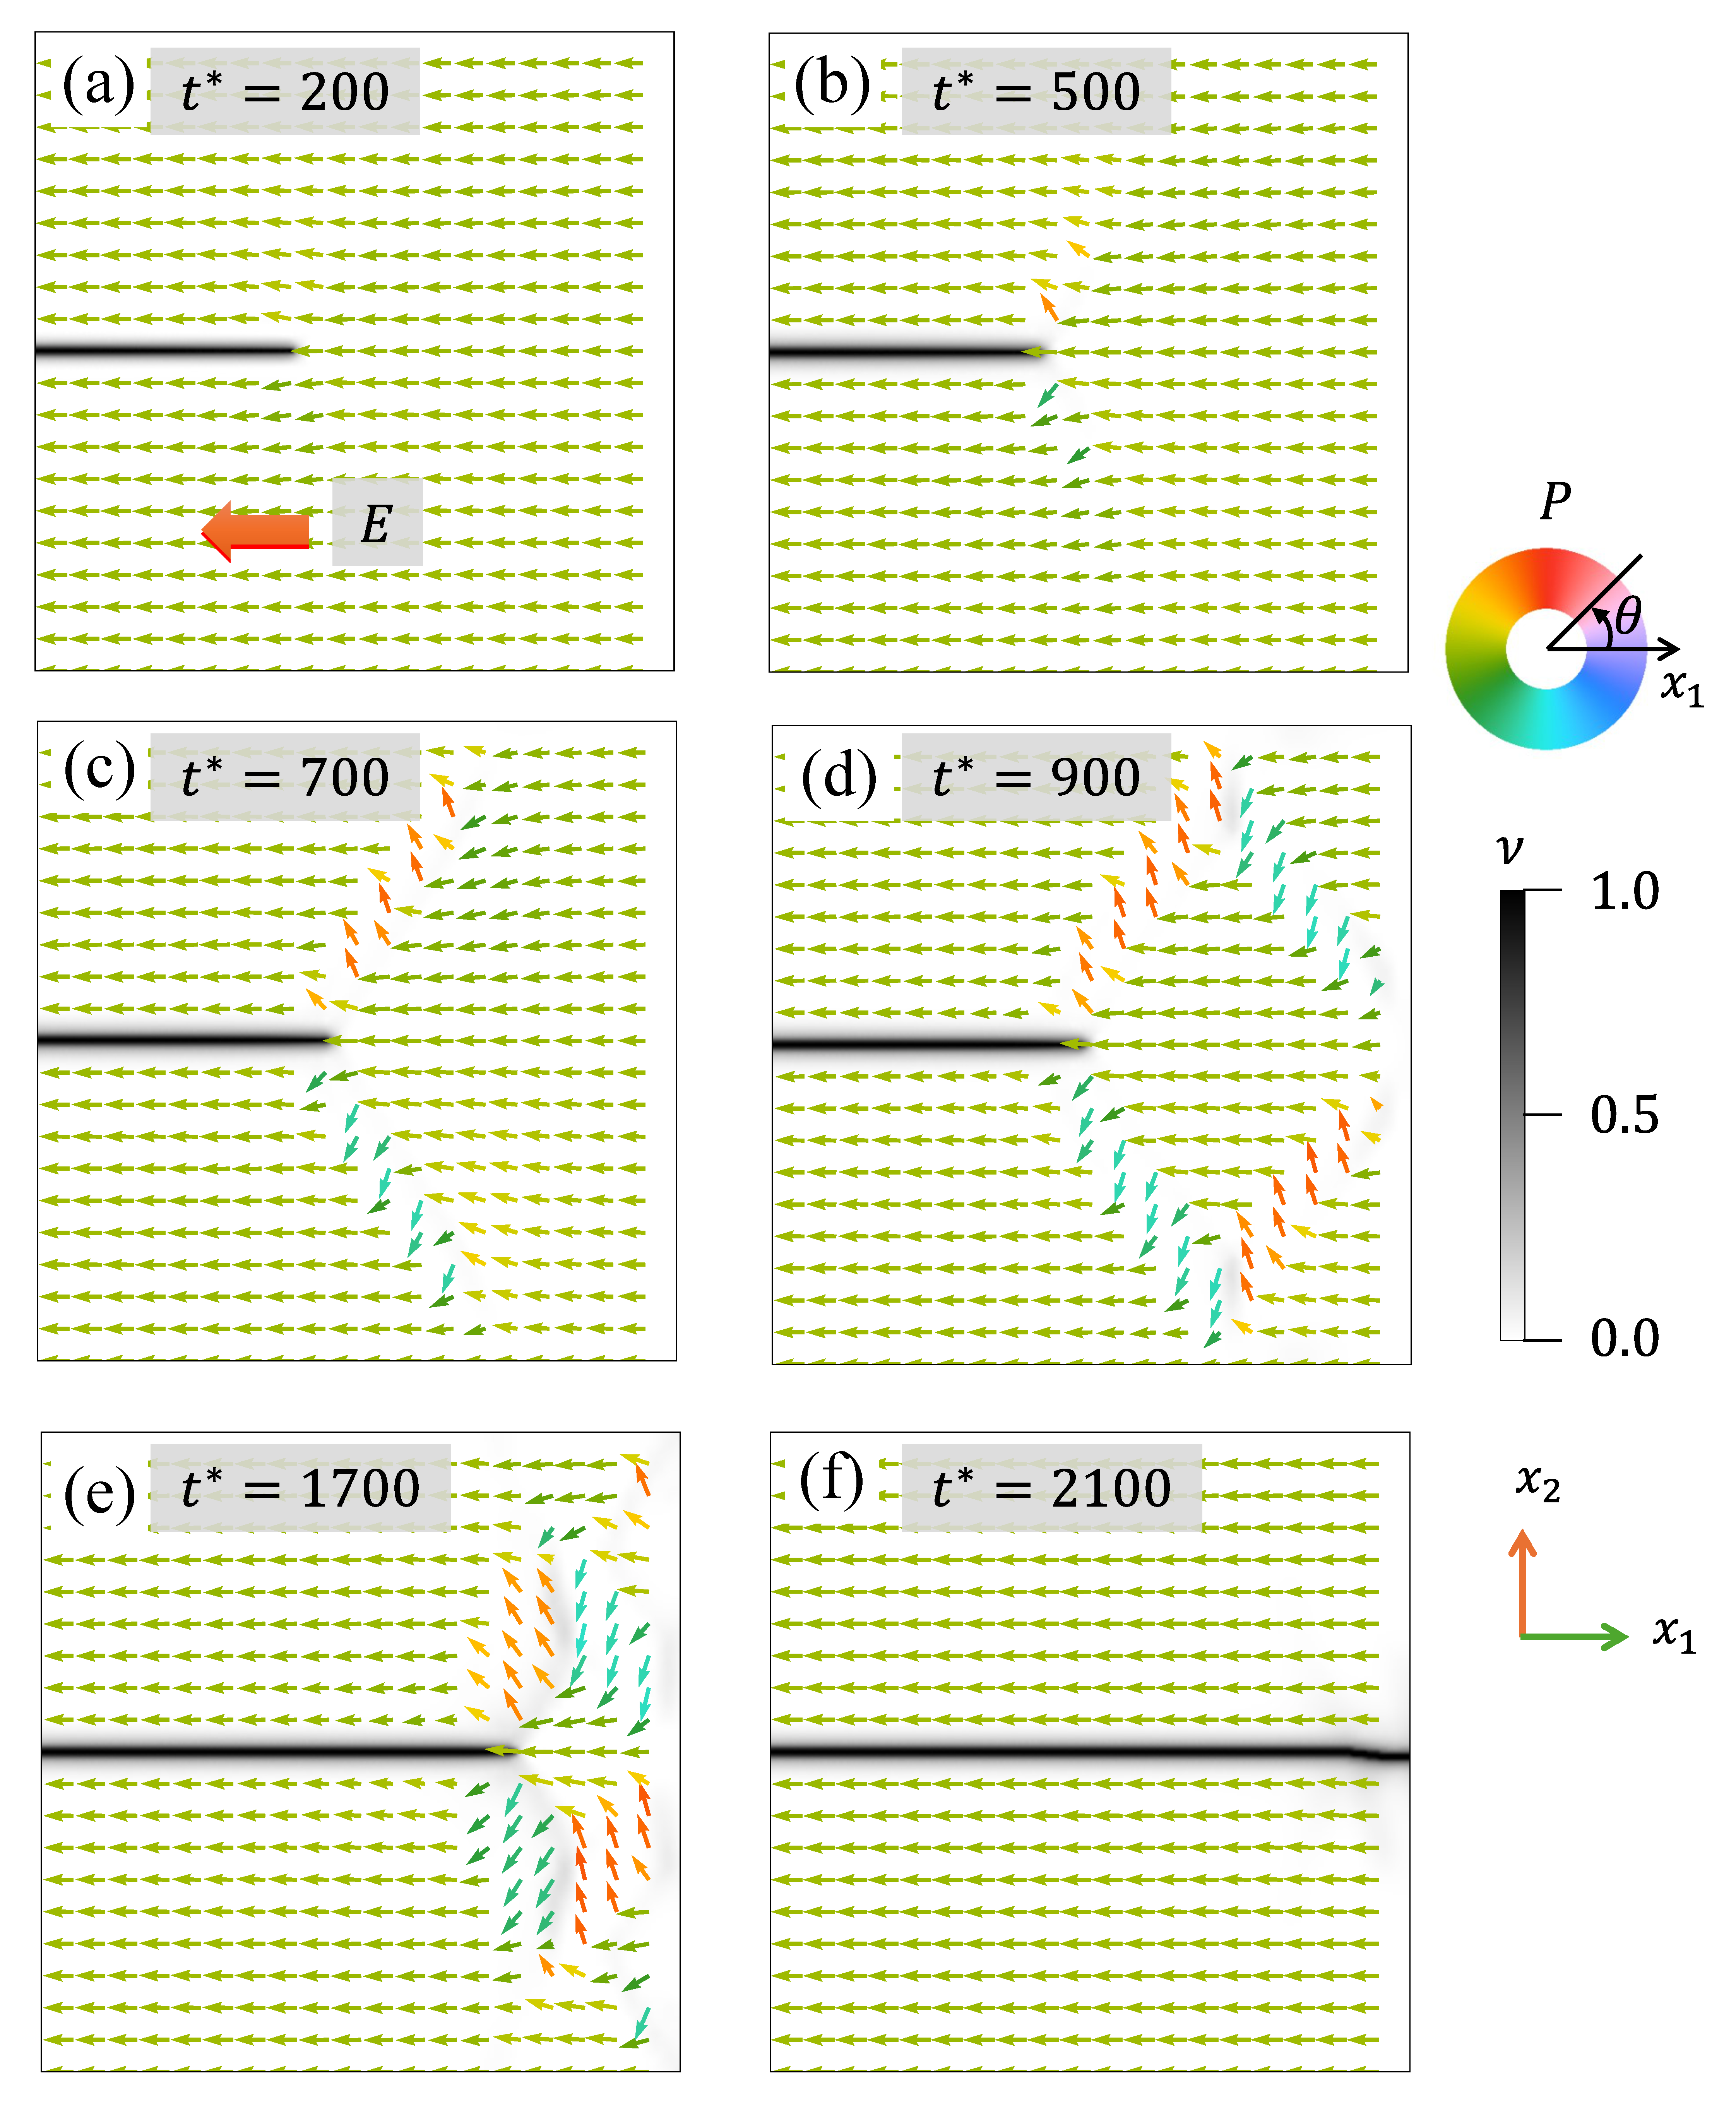
\includegraphics[width=\linewidth]{Fig3.pdf}
    \caption{Morphologies of the crack and polarization at various moments $t^*=200$, 500, 700, 900, 1700, and 2100 under the applied electric field $E^*_1=-1$, respectively. Here, the flexoelectric effect is neglected.} \label{fig3}
\end{figure}

As a comparison, Figure \ref{fig3} illustrates the evolution of the crack and domain structure under an external load with the initial polarization opposing the $x_1$-axis. Similarly, the flexoelectric coefficients $f_{ij}$ are set to zero. The results at time steps $t^*=$200, 500, 700, 900, 1700, and 2100 show that both the length of crack propagation and the polarization evolution are identical with the case where polarization directions align along the $x_1$-axis. The difference lies in the polarization direction being opposite to the corresponding positions in Figure \ref{fig2}. The results indicate that, in the absence of the flexoelectric effect, as long as the polarization direction is parallel to the crack, the fracture process in ferroelectric materials remains consistent. The full spatial and temporal evolution of the domain structure and crack path are shown in Video S2.

Figure \ref{fig4}(a) illustrates the variations of crack extension length $\Delta x$ and the rate $\mathrm{d}\Delta x/\mathrm{d} t$ as functions of $t$ when the initial polarization is parallel to the crack. In the absence of the flexoelectric effect, the crack extension rate is identical in both cases where the initial polarization is oriented in the left or right direction. At $t^*=379$, which corresponds to the displacement load $u_y^*=0.794$, the crack begins to extend. From $t^*=400$ to $t^*=900$, the crack tip moves forward at a steady rate. Beyond the time step $t^*=900$, the crack extension rate increases rapidly, leading to an  accelerated crack propagation until complete fracture occurs.

To quantify the driving force for crack propagation in ferroelectric materials, the concept of configurational force is employed \cite{kuhn_discussion_2016}:
\begin{equation}
    \mathbf{g}_\mathrm{frac}=-\nabla\cdot\left( \psi_\mathrm{{frac}}\mathbf{I}-\nabla\nu\otimes\frac{\partial\psi}{\partial\nabla\nu} \right),
\end{equation}
\begin{equation}
    \mathbf{g}_{d}=-\frac{\dot{\nu}}{L_\nu}\nabla\nu,
\end{equation}
where the symbol $\mathbf{I}$ denote the 2nd-rank unit tensor. The terms $\mathbf{g}_\mathrm{frac}$ and $\mathbf{g}_d$ represent the resistance and net driving force for fracture, respectively. Aligning the concept of fracture configurational force with the $J$-integral, the summation of the $x_1$ components of $\mathbf{g}_\mathrm{frac}$ and  $\mathbf{g}_d$ can be represented by $J_c$ for the local fracture toughness, and by $J$ for the driving force, as detailed by Zhang et al.\cite{yong_zhang_phase_2022,zhang_jumping_2022}. The region for calculating $J$ and $J_c$ is selected by a circle centered at the crack tip, with a radius of 5, as illustrated in Figure \ref{fig1}(b).

\begin{figure}[!htbp]
    \centering
    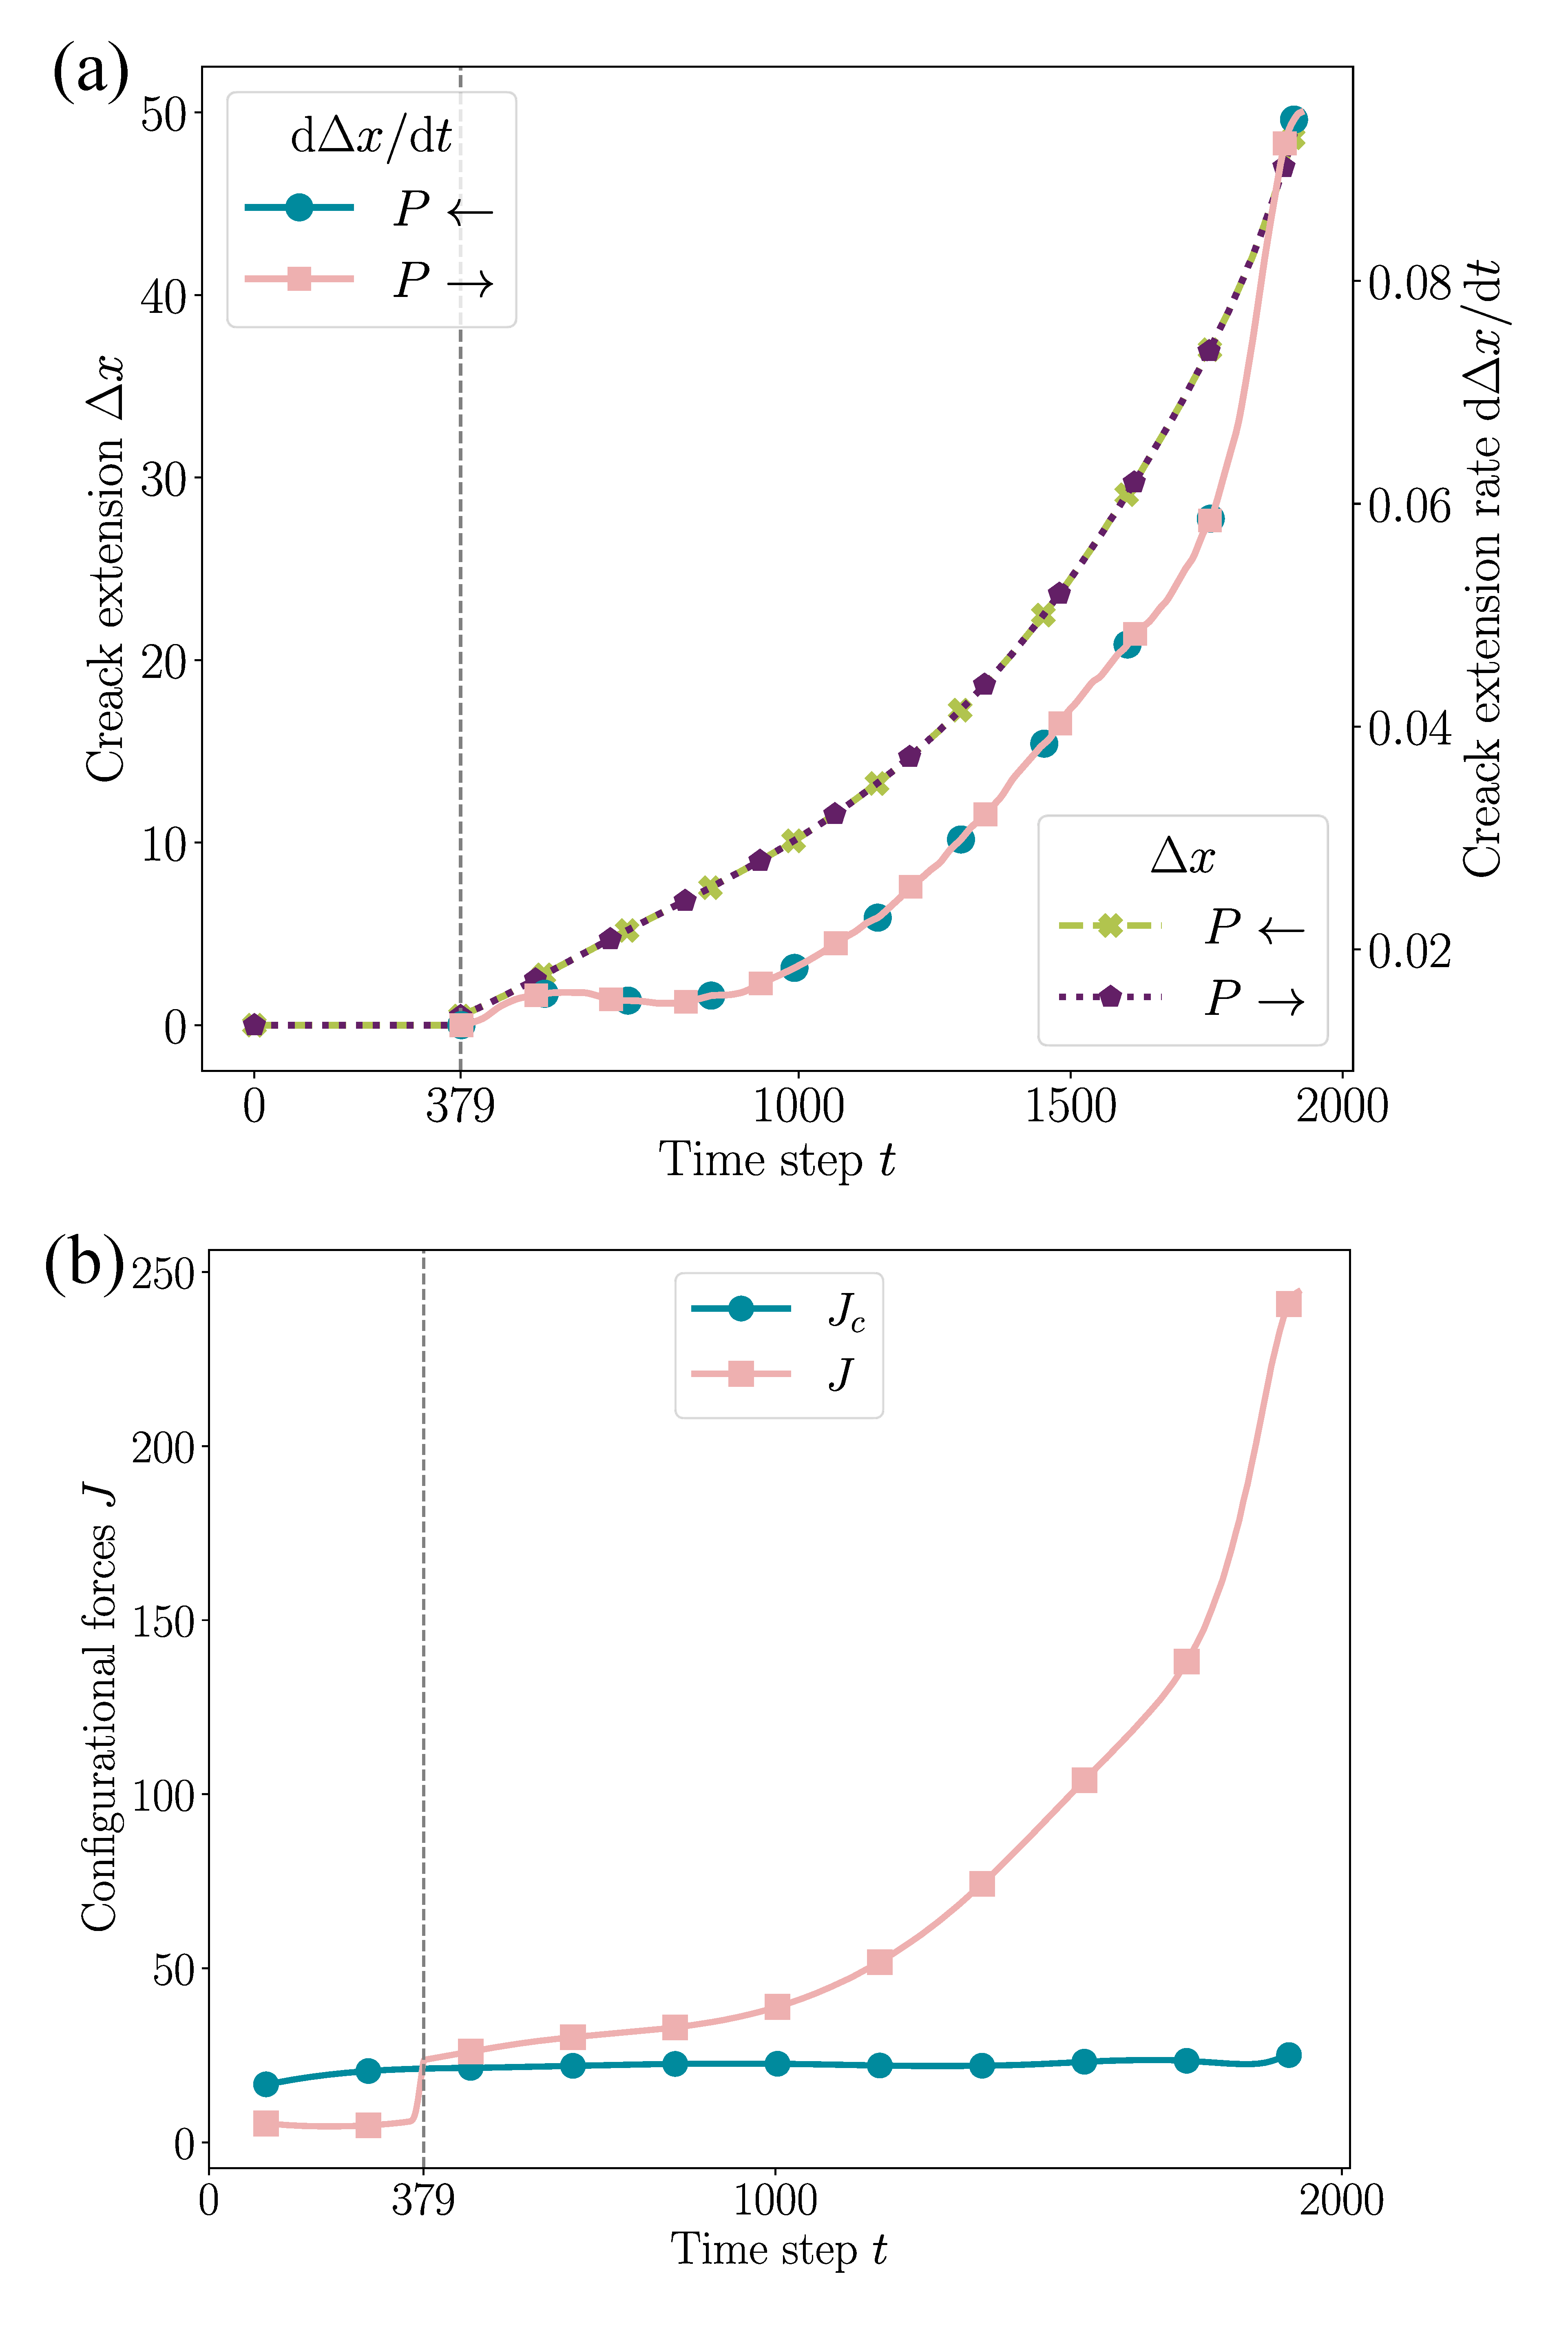
\includegraphics[width=0.7\linewidth]{Fig4.pdf}
    \caption{(a) The variation of crack extension $\Delta x$ (left $y$-axis) and the crack extension rate $\mathrm{d}\Delta x/\mathrm{d}t$ (right $y$-axis) with respect to the time step $t$. The arrows in the legend indicate the initial direction of polarization. Solid lines represent crack extension $\Delta x$, while dashed lines corresponding to the crack extension rate $\mathrm{d}\Delta x/\mathrm{d}t$; (b) The change of the crack extension driving force $J$ and local fracture toughness over time step $t$.} \label{fig4}
\end{figure}

Figure \ref{fig4}(b) shows the variation of the crack driving force $J^*$ and the resistance $J_c^*$ over time steps with $f_{ij}=0$. Throughout the entire crack propagation process, the resistance $J_c^*$ remains consistently stable at around 20, closely approximating the critical fracture toughness value of $G_c^*=20.2$.  Prior to the onset of crack propagation, the crack driving force $J^*$ is lower than the resistance $J_c^*$. As the applied displacement load $u_y^*$ continues to increase, $J^*$ exceeds $J_c^*$ at time $t^*=379$, triggering the start of crack growth. As the crack progresses from $t^*=400$ to $t^*=900$, new domain walls are established near the crack tip, as shown in Figure \ref{fig2} and Figure \ref{fig3}. During this period, the energy is allocated not only to the propagation of the crack but also to the generation of domain walls. This leads to a competition between $\psi_\mathrm{grad}$ and $\psi_\mathrm{frac}$, decelerating the crack extension rate, which is referred to as the polarization switching-induced toughening effect \cite{wang_phase_2007}. In the absence of new domain wall formation after $t^*>900$, the competition between $\psi_\mathrm{grad}$ and $\psi_\mathrm{frac}$ dissipates. Furthermore, the polarization switched zone continuously diminishes as the crack propagates, leading to a rapid increase in the $J^*$. This in turn causes the crack propagation rate to continually rise until complete fracture.

\begin{figure}[!htbp]
    \centering
    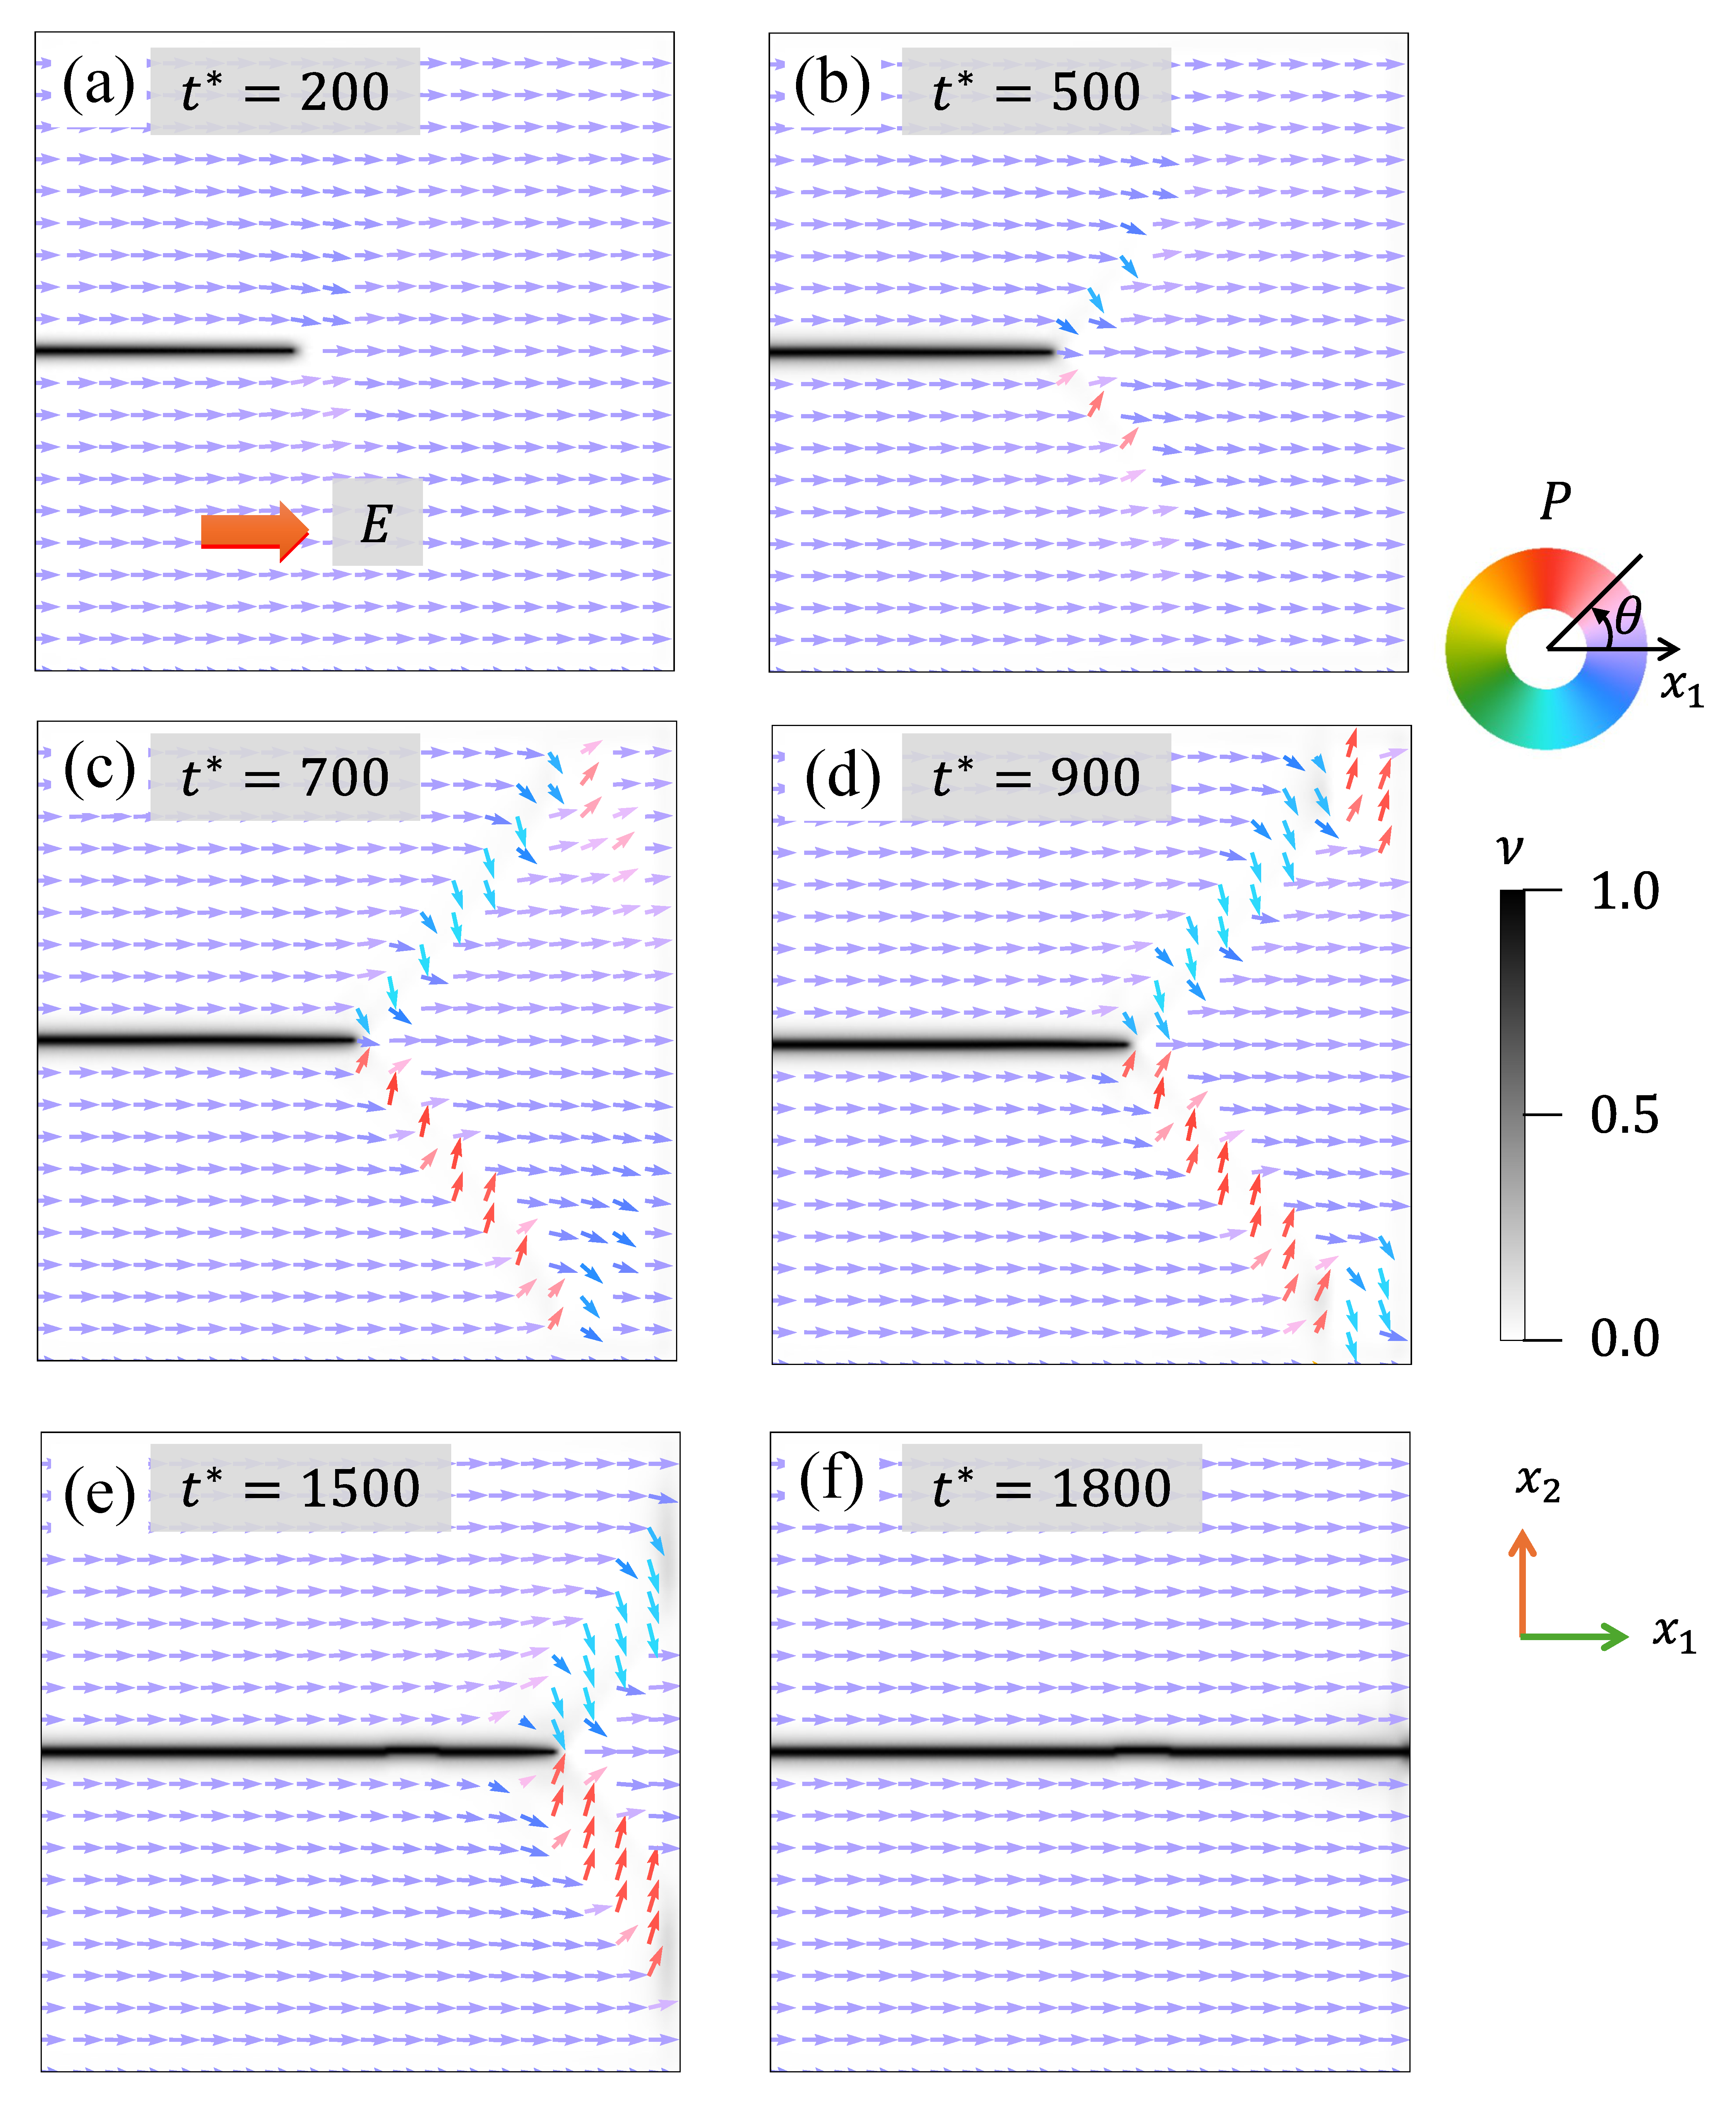
\includegraphics[width=\linewidth]{Fig5.pdf}
    \caption{Morphologies of the crack and polarization at various moments $t^*=200$, 500, 700, 900, 1500, and 1800 under the applied electric field $E^*_1=1$, respectively. The flexoelectric effect is incorporated here.} \label{fig5}
\end{figure}

With the flexoelectric effect, the fracture behaviors in ferroelectric materials undergo noticeable changes. Figure \ref{fig5} presents the evolution of the crack path and domain structure in a ferroelectric plate across various time steps with the flexoelectric effect. The initial direction of polarization is oriented in the right direction. Similarly, before crack propagation, only the polarization near the crack tip undergoes rotations of less than $45^\circ$ without forming a distinct switched zone, as shown in Figure \ref{fig5}(a). Once the crack begins to extend, a switched zone with two forward wings also forms near the crack tip, as depicted in Figure \ref{fig5}(b) and (c). However, in contrast to the results in Figure 2, when the foremost area of the switched zone reaches the edge of the plate, the length of crack extension is significantly longer than the counterpart without the flexoelectric effect. Consequently, the front of the newly formed switched zone reaches the right edge of the plate, which is unable to form a complete diamond structure, as shown in Figure \ref{fig5}(d). As the crack continues to propagate, the two forward wings on both sides of the crack tip move forward, while the newly formed switched zone continually shrinks until it disappears, as illustrated in Figure \ref{fig5}(e). Once the plate is completely fractured, the polarization returns to a single domain state, as presented in Figure \ref{fig5}(f). The complete evolution process of the domain structure and crack path is presented in Video S3.

Figure \ref{fig6} demonstrates the case where the initial polarization is opposite to the crack propagation with the consideration of the flexoelectric effect. As shown in Figure \ref{fig6}(a), prior to crack extension, the entire ferroelectric material maintains a single domain state with polarization aligned along the left direction, which is consistent with the direction of the electric field. With the crack extension, a $90^\circ$ rotation of polarization occurs on both sides of the crack tip, as depicted in Figure \ref{fig6}(b). This leads to the emergence of two symmetrical forward wings structures, with opposite polarization directions on each side. By the time $t^*=900$, the $90^\circ$ polarization switched zones develop on either side of the tips of the forward wings structure, leading to the formation of domain structures. Then compared to other cases, the ferroelectric material contains more domain walls, as displayed in Figure \ref{fig6}(c). At $t^*=1600$, the regions of polarization switching also evolve into diamond structures. However, unlike in other cases, the polarization switching zones started behind the crack tip rather than at the crack tip, as shown in \ref{fig6}(d). As the crack tip gradually approaches the right edge, the diamond structure vanishes, and the polarization switching region at the crack tip transforms into a backward wing structure. This structure maintains symmetrical in both morphology and polarization direction relative to the crack plane, with symmetrical auxiliary wing-like structures forming on both the upper and lower sides, as shown in Figure 6(e). The complete spatial and temporal evolution of the domain structure and crack path is presented in Video S4.

\begin{figure}[!htbp]
    \centering
    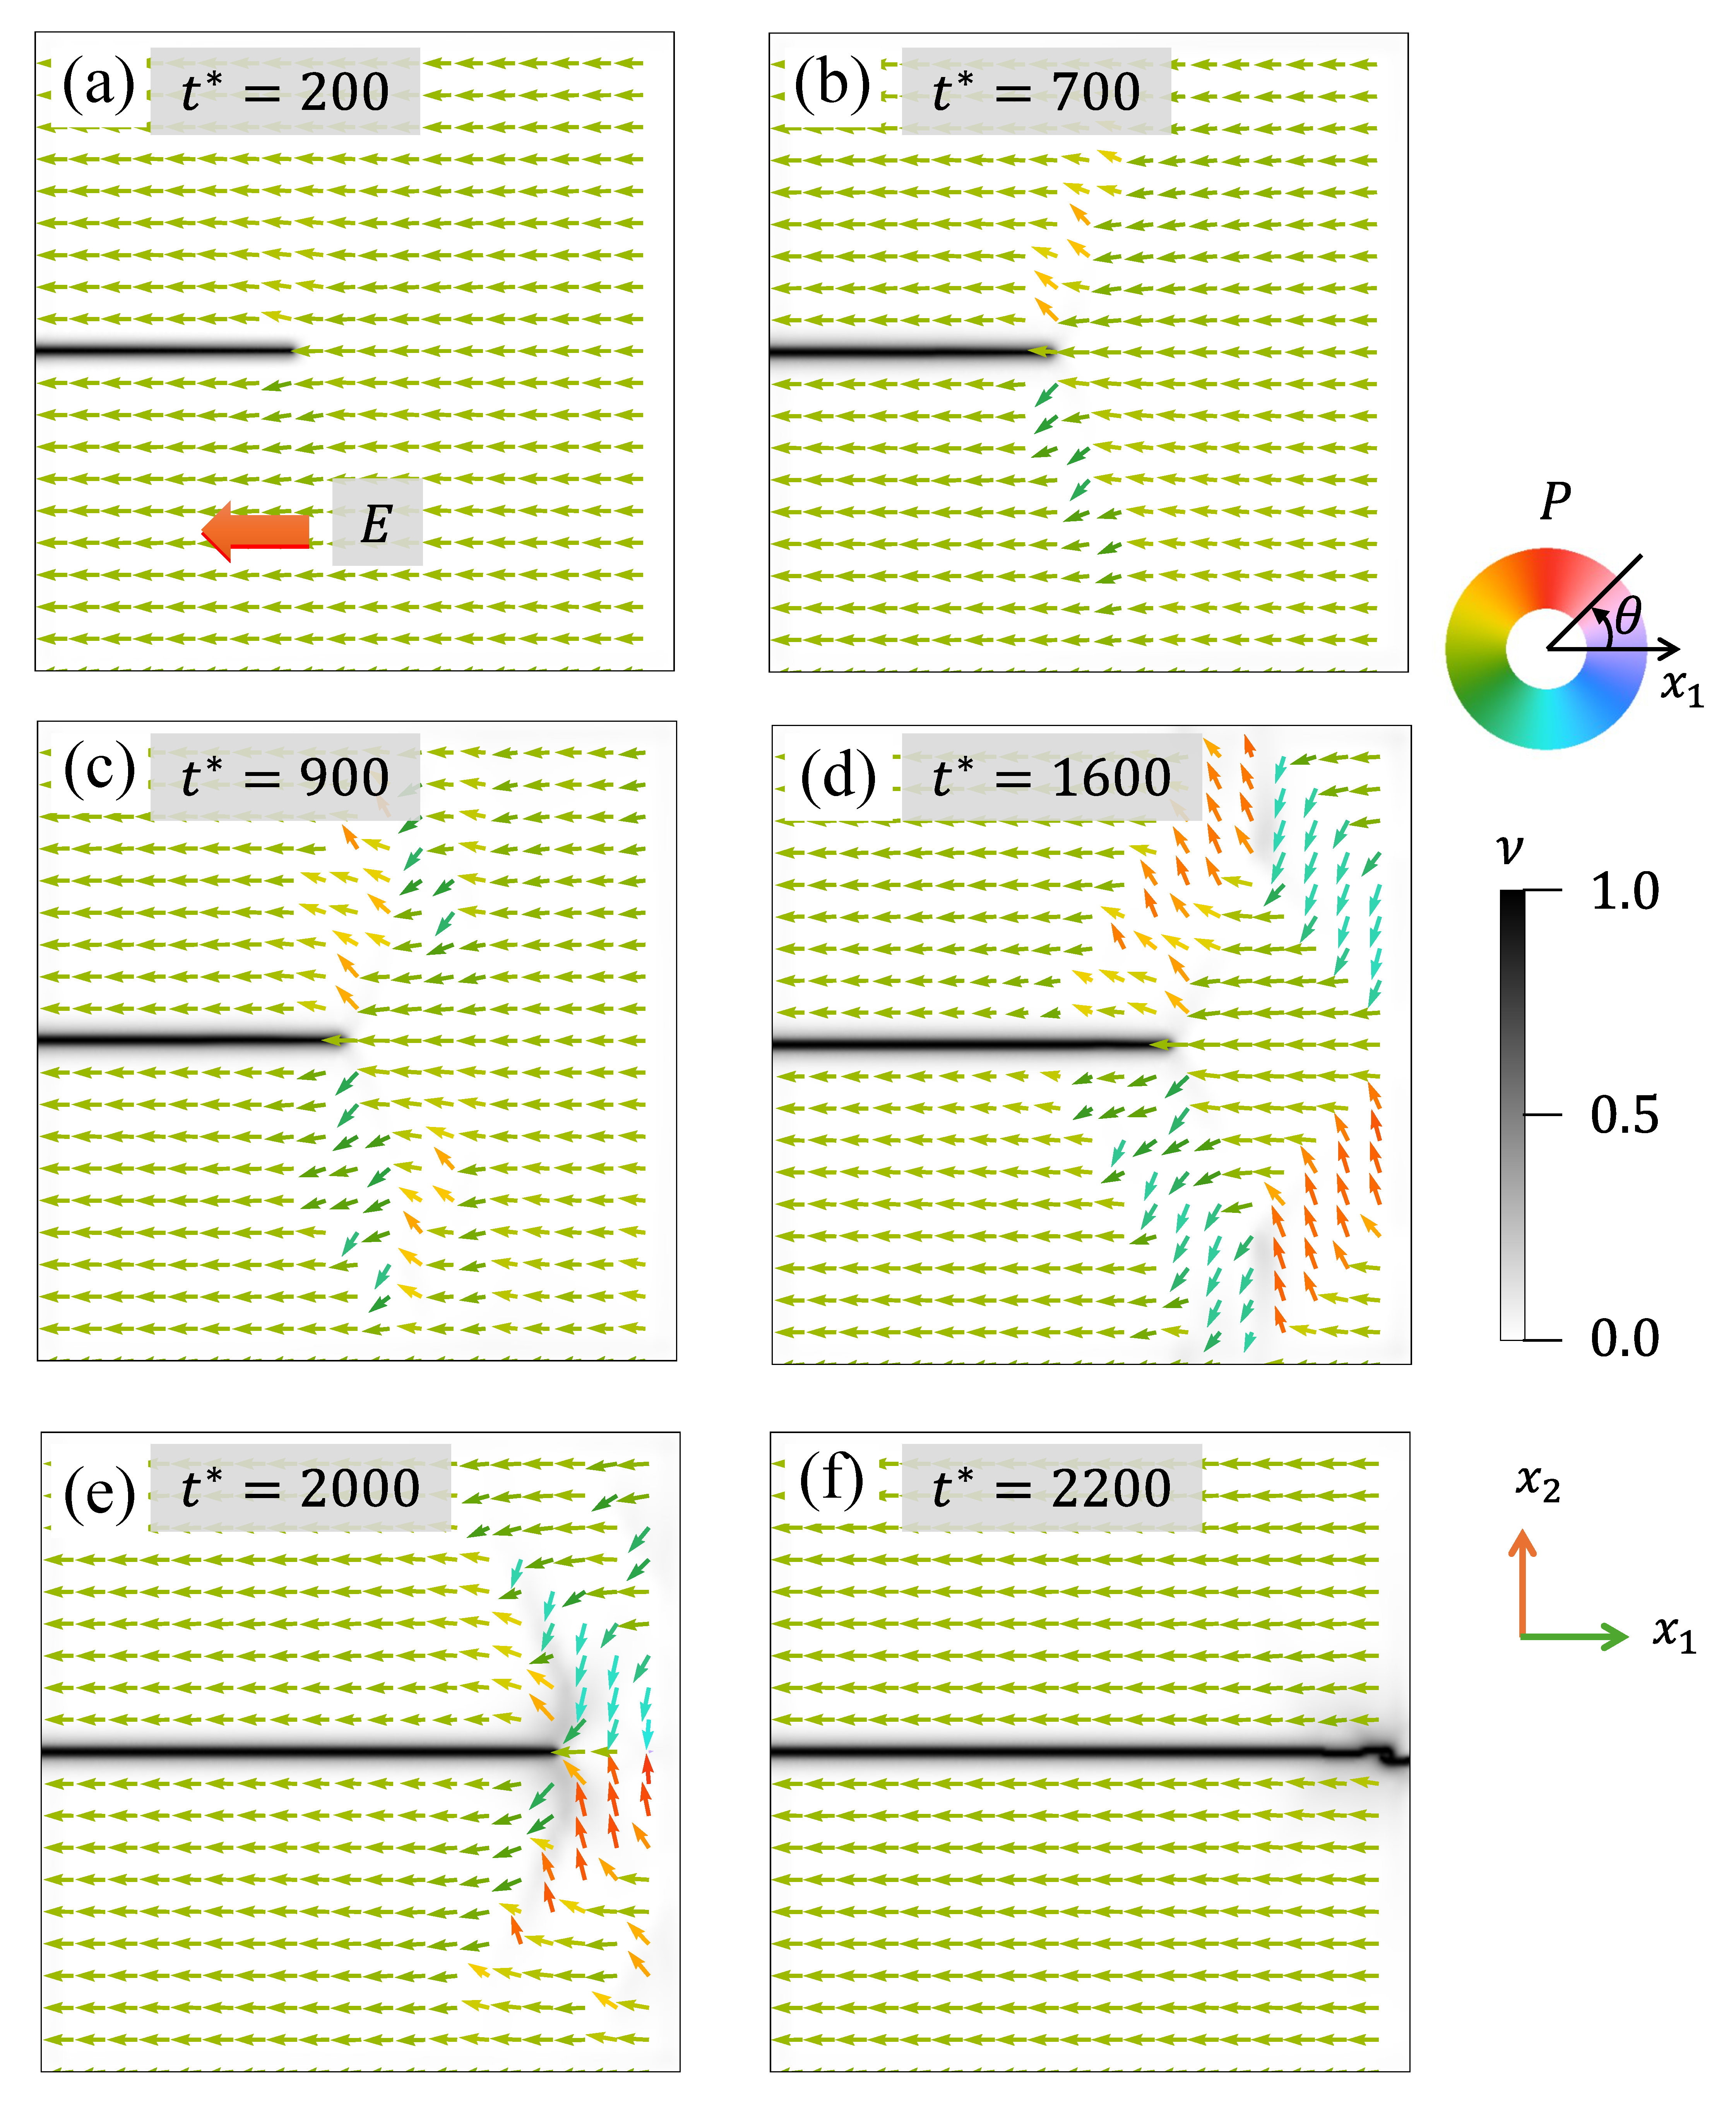
\includegraphics[width=\linewidth]{Fig6.pdf}
    \caption{Morphologies of the crack and polarization at moments $t^*=200$, 700, 900, 1600, 2000, and 2200 under the applied electric field $E^*_1=-1$, respectively.} \label{fig6}
\end{figure}

Figure \ref{fig7}(a) illustrates the crack extension $\Delta x$ over time step $t$. When considering the flexoelectric effect, if the polarization direction coincides with the direction of crack propagation, the crack extends earlier and requires a lower external load, consequently diminishing the material's fracture toughness. However, when the crack propagation direction is opposite to the polarization direction, the extension of the crack is delayed and requires a larger external load to initiate propagation, effectively increasing the material's fracture toughness. Thus, the flexoelectric effect can lead to asymmetric fracture toughness of ferroelectric materials. This numerical result is accordance with the previous experimental observation \cite{cordero-edwards_flexoelectric_2019}.

\begin{figure}[!htbp]
    \centering
    \includegraphics[width=\linewidth]{Fig7.pdf}
    \caption{(a) the change in crack extension length over time step $t$. Arrows in the figure indicate the direction of initial polarization, solid lines with markers represent data considering the flexoelectric effect, and dashed lines represent data without the flexoelectric effect. (b) the change in $\varepsilon_{22}^{\mathrm{eige}}$ along $y=50$, from the crack tip to the right boundary of the plate at $t=200$. (c) and (d), the distribution of eigenstrain $\varepsilon_{22}^{\mathrm{eige}}$ near the crack tip, in which the arrows represent the direction of initial polarization, respectively. The dashed lines in the images mark the region of the crack ($\nu\geq0.9$). } \label{fig7}
\end{figure}

With the presence of the flexoelectric effect, the polarization gradient $\nabla \mathbf{P}$ induces an additional eigenstrain $\mathbf{\varepsilon}^{\mathrm{flex}}$ \cite{gu_phase-field_2014}:
\begin{equation}
    \varepsilon_{yy}^{\mathrm{eige}}=-F_{11}\frac{\partial P_y}{\partial y}-F_{12}\frac{\partial P_x}{\partial x},
\end{equation}
in which $F_{ij}=s_{ik}f_{kj}$, and $s_{kj}$ are the compliance coefficients. The polarization gradient induced eigenstrain $\varepsilon_{22}^{\mathrm{eige}}$ is concentrated on the crack tip, corresponding to the opposite polarization rotation on the two sides of the crack tip. As depicted in Figure \ref{fig7}(b), the polarization gradient generates a positive eigenstrain $\varepsilon_{22}^{\mathrm{eige}}$ at the crack tip due to the flexoelectric effect. This additional positive strain increases the strain concentration at the crack tip, consequently accelerating crack propagation. Conversely, when the polarization is oriented in the left direction, the eigenstrain $\varepsilon_{22}^{\mathrm{eige}}$ become negative at the crack tip, effectively producing an additional compression, as shown in Figure \ref{fig7}(d). This reduces the strain concentration at the crack tip and delays the crack propagation.

In addition, according to Hwang's research \cite{hwang_ferroelectricferroelastic_1995}, the domain switching should satisfy:
\begin{equation}
    \sigma_{ij}\Delta \varepsilon_{ij}+E_i\Delta P_i \geq 2P_S E_C,
\end{equation}
where $P_S$ and $E_C$ denote the magnitude of the spontaneous polarization and coercive field, respectively. Thus, the additional eigenstrain also impacts the formation of domain walls. In the cases where the polarization direction aligns along the right direction, a positive $\varepsilon_{22}^{\mathrm{eige}}$ facilitates the rotation of polarization and the earlier formation of domain structures. On the other hand, when the polarization direction is opposite to the crack propagation direction, a negative $\varepsilon_{22}^{\mathrm{eige}}$ requires a larger load to achieve polarization rotation and domain structure formation.

The coupling between domain evolution and flexoelectric effect can significantly influence the fracture driving force $J$. As presented in Figure \ref{fig8}, the crack driving force $J$ is higher for the initial polarization oriented in the right direction in the early stages of crack propagation. Due to the larger tensile strain at the crack tip and fewer domain walls, more energy is dedicated to driving crack growth. As the crack further extends, by the time $t^*>1500$, the cases where the polarization direction is along the left direction exhibit longer undamaged regions. Under the same displacement load $u_y$, it will endure larger stress. Additionally, as the crack extends, the domain walls begin to vanish, releasing energy and further accelerating crack propagation. Consequently, at this stage, the cases with the polarization direction aligned in the left direction have a larger driving force $J$.

\begin{figure}[!htbp]
    \centering
    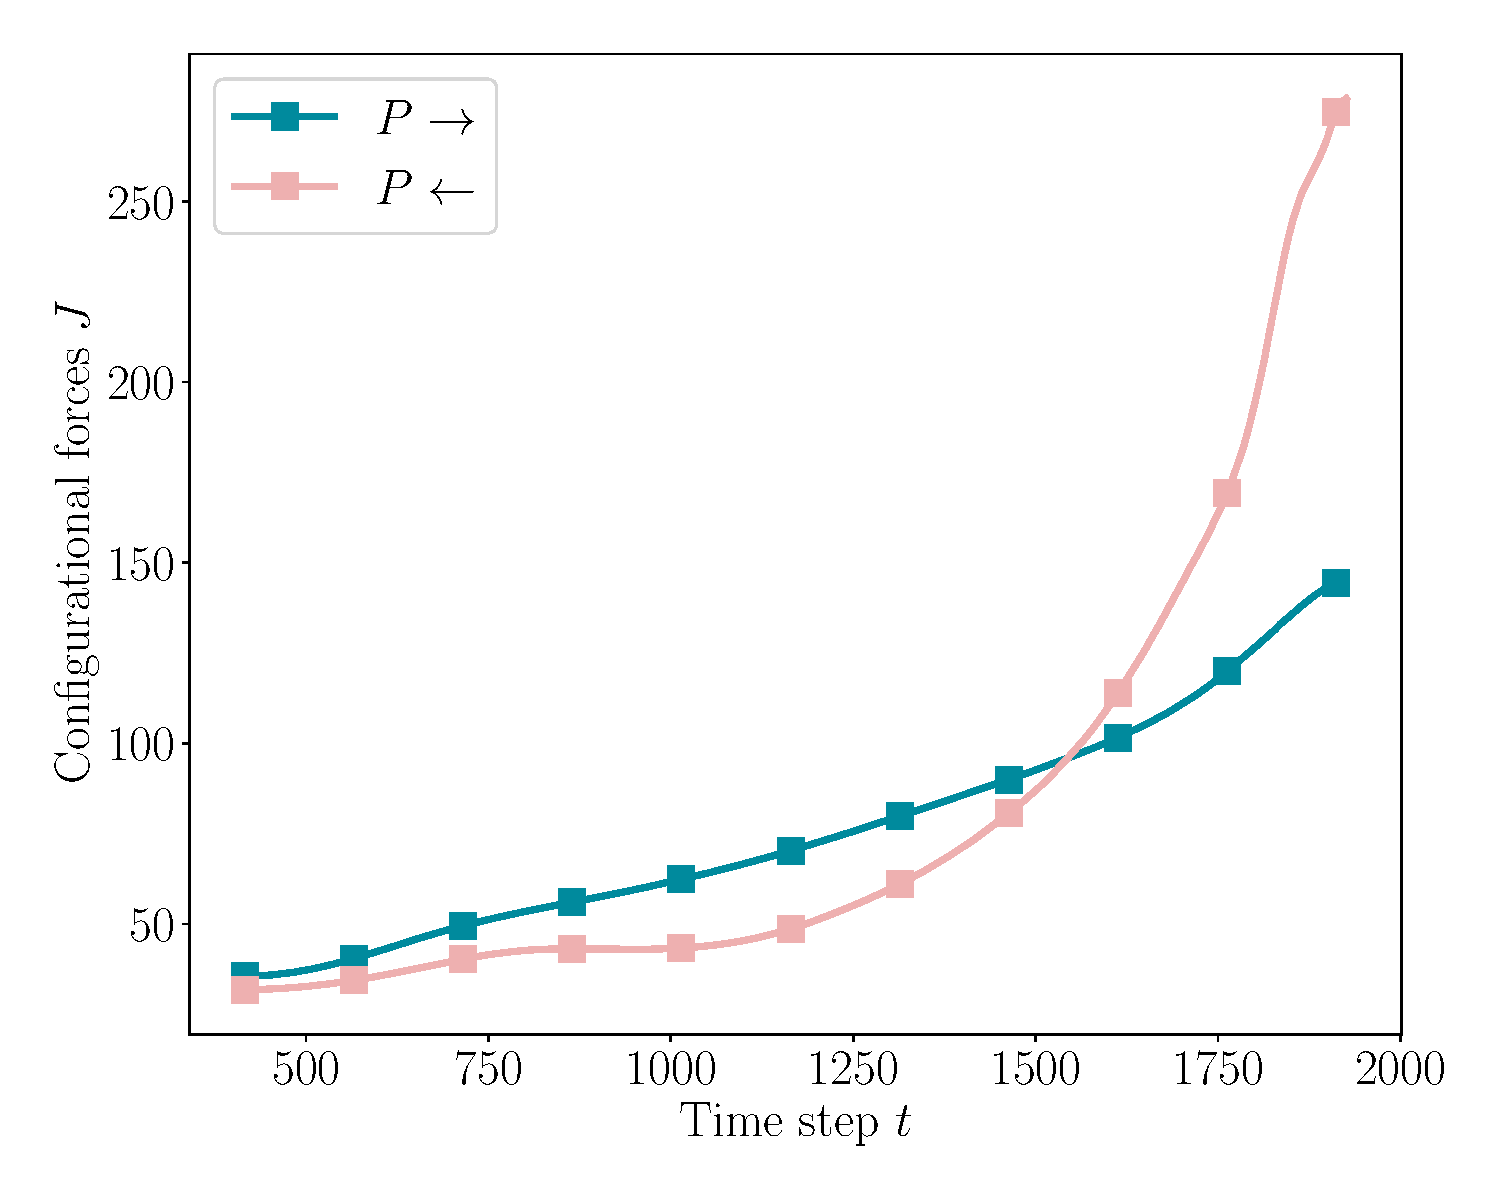
\includegraphics[width=0.7\linewidth]{Fig8.pdf}
    \caption{The variation of  fracture driving force $J$  over time step $t$.} \label{fig8}
\end{figure}

\subsection{Crack perpendicular to the initial polarization direction}

Figure \ref{fig9} illustrates the temporal evolution of the polarization domain structure and crack propagation in ferroelectric material. Here, the flexoelectric effect is neglected, and the electric field $E_2^*=-1$ is applied to the ferroelectric material. As shown in Figure \ref{fig9}(a), on either side of the crack, the polarization rotates $90^\circ$ in counterclockwise and clockwise direction, respectively. This results in the formation of two switched zones with forward wings structure in the material. Along the side of these wings, $90^\circ$ domain walls are formed. The tips of the wings extend to the right boundary of the plate, effectively segmenting the unswitched area into three triangular zones. Distinct from cases where the crack is aligned parallel to the initial polarization direction, domain structures are already present within the plate before crack propagation. According to Eq.\eqref{eq5}, the polarization component $P_2$ can induce a positive spontaneous strain $\varepsilon^0_{22}$.  This fundamental relationship suggests that the initial displacement load $u_2=0$ effectively introduces an additional compressive force. Besides, due to the electrical impermeability of the crack, the electric field continuity across the pre-existing  crack is disrupted. Hence, domain walls are established even prior to crack propagation.

As $u_2$ increases, the crack begins to extend. Under the influences of $u_2$ and $E_2$, the polarization in the switched zones gradually rotates to align with the direction of the electric field. Consequently, the forward wing structure progressively diminishes, as shown in Figure \ref{fig9}(b)-(c). At $t^*=2500$, the two forward wings structure has completely vanished. At this point, the polarization distribution within the material is divided into two parts by the crack tip. On the right side of the plate, where the material is intact, the polarization remains almost a single-domain state, with polarization aligned along the electric field. On the left side, an antisymmetric domain structure forms on both sides of the crack, which comprises $180\circ$ and $90^\circ$ domain walls, as presented in Figure \ref{fig9}. As $u_y$ continues to increase, the crack further extends. Two continuous polarization vortices form on either side of the crack plane, which is listed in Figure \ref{fig9}(e). After fully fractured, the plate does not revert to a single-domain state. Instead, a flux closure structure is formed on both sides of the crack, as shown in Figure \ref{fig9}{f}. Given that the crack is electrically impermeable, the areas of electrical discontinuity increase as the crack extends. Once the crack has fully extended, the regions above and below the crack effectively become open-circuited. Consequently, under the influence of external forces, the domain structures no longer revert to a single-domain state. The complete spatial and temporal evolutions of the domain structure and crack path are presented in Video S5.

\begin{figure}[!htbp]
    \centering
    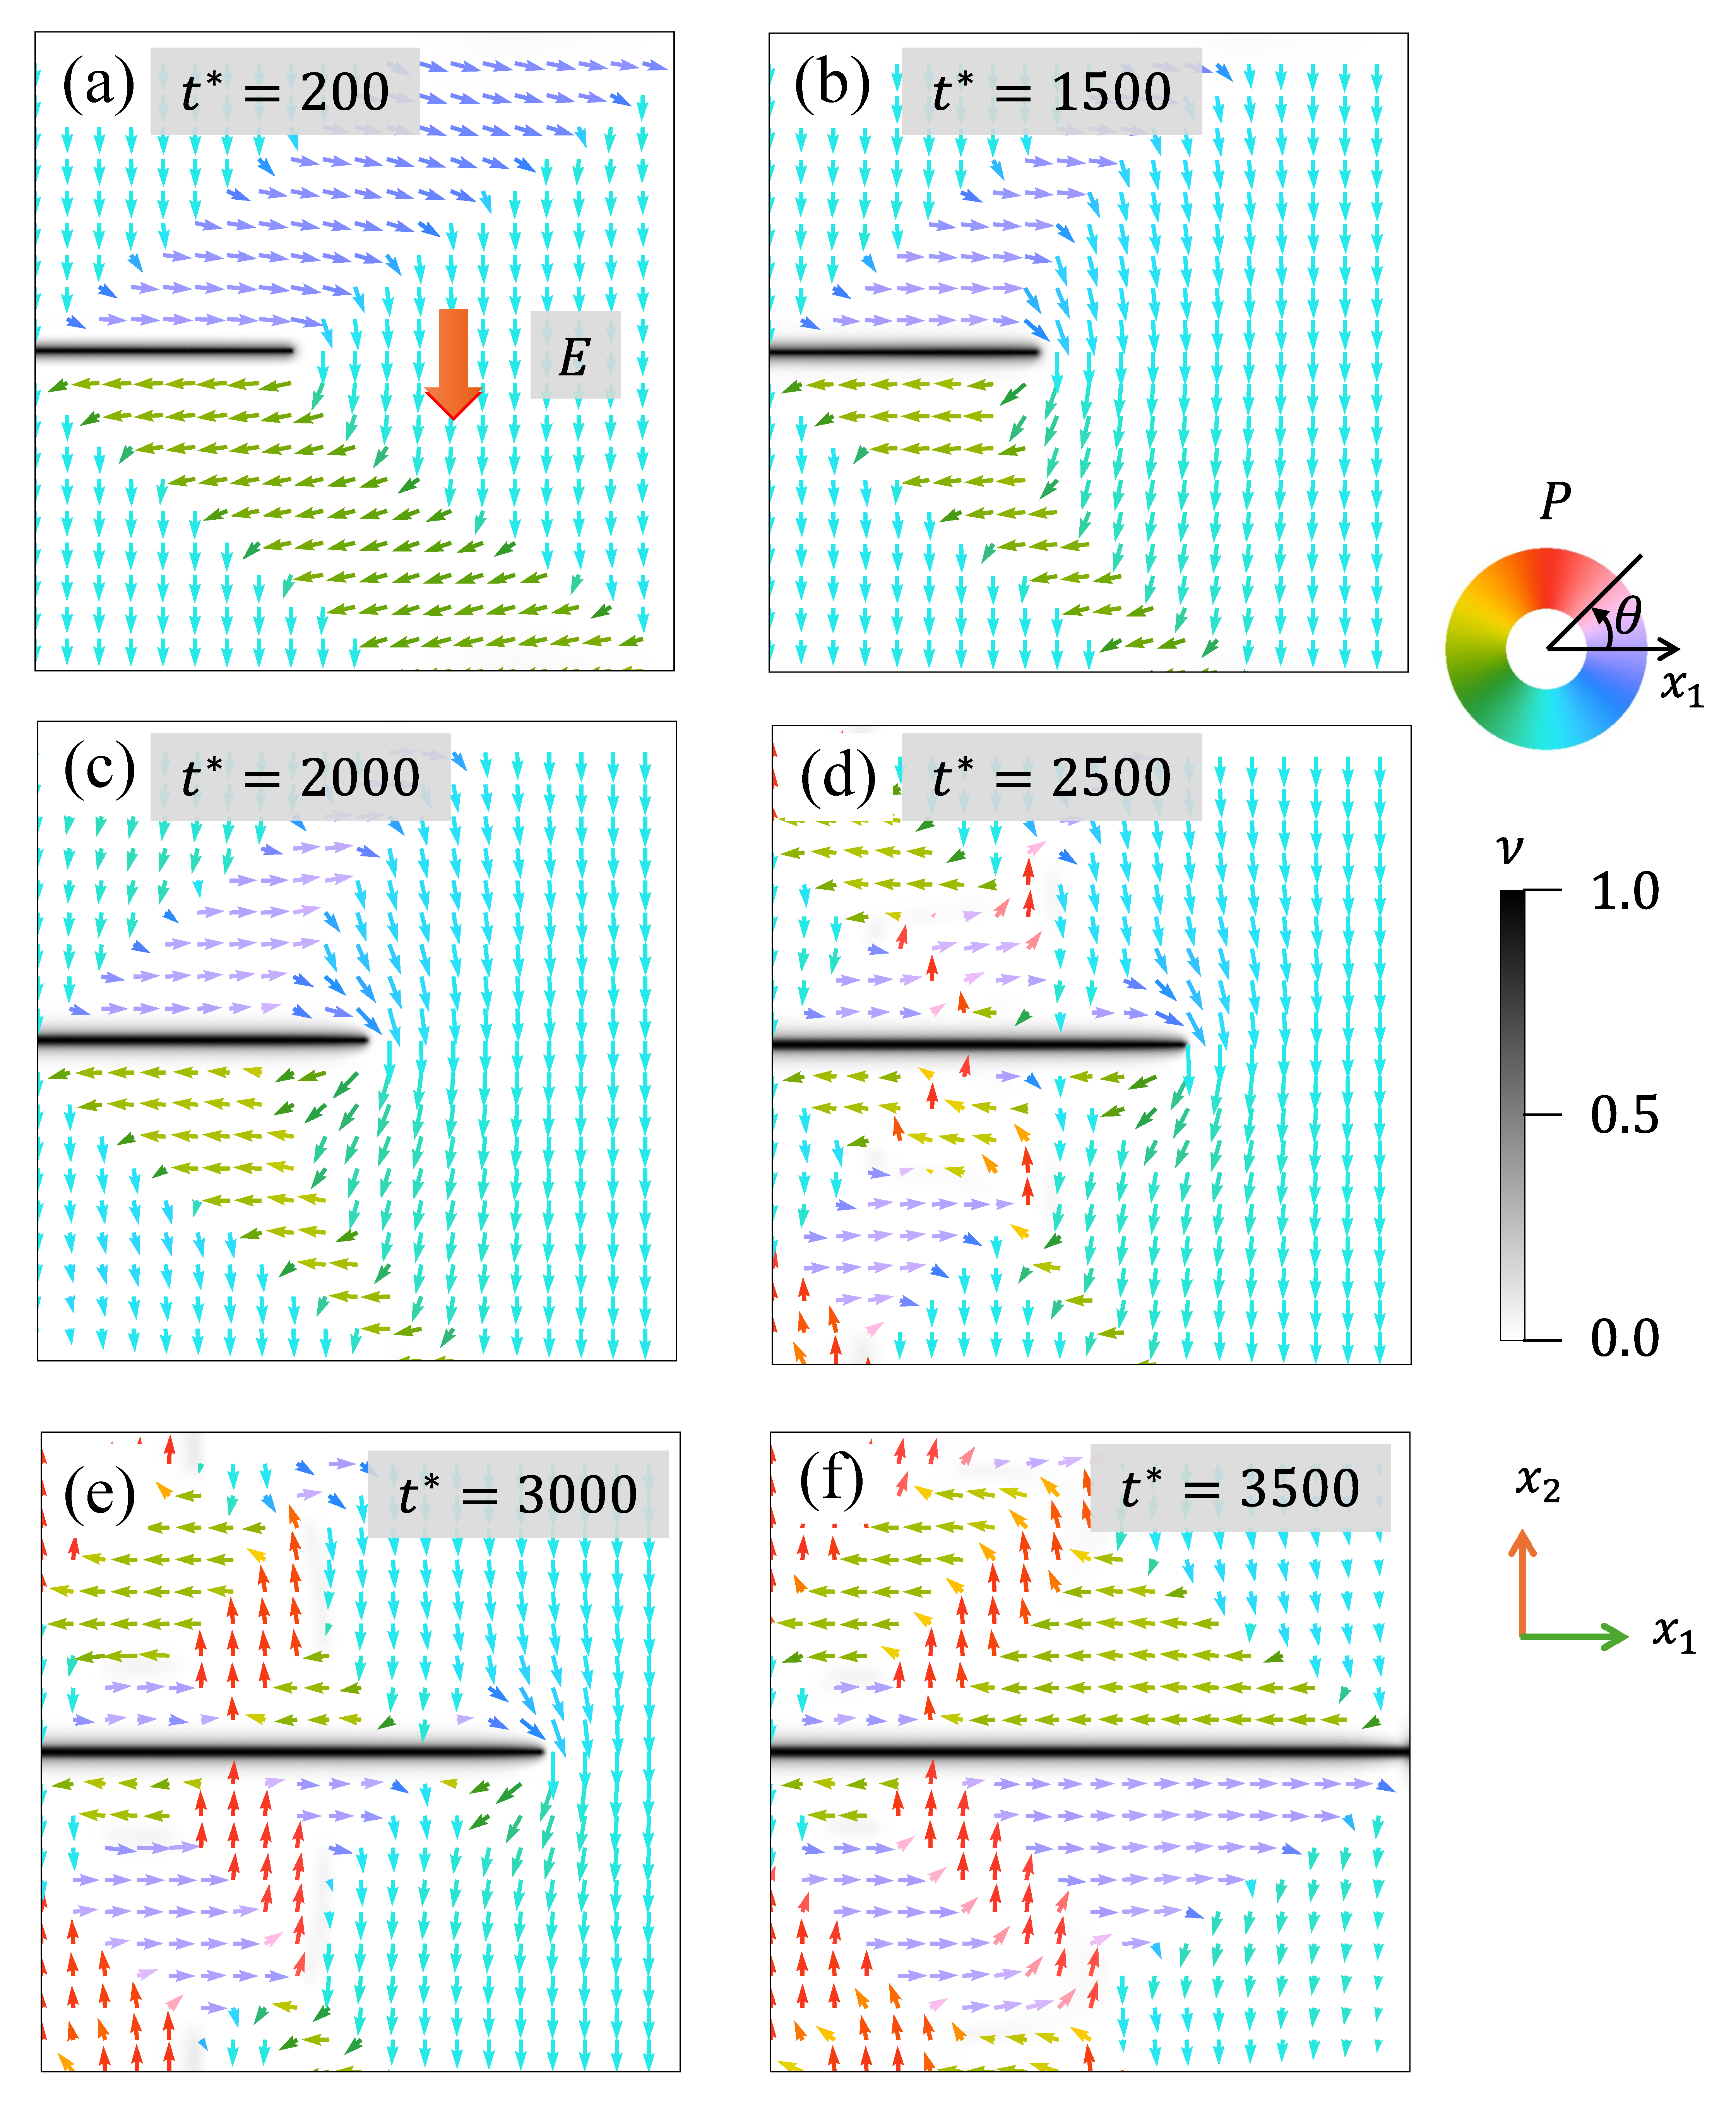
\includegraphics[width=\linewidth]{Fig9.pdf}
    \caption{The dynamic progression of crack propagation and polarization switching at time step $t^*=200$, $t^*=1500$, $t^*=2000$, $t^*=2500$, $t^*=3000$ and $t^*=3500$. The grayscale maps illustrate the spatial distribution of the fracture order parameter $\nu$. The arrows indicate the orientation and magnitude of the polarization vectors. The flexoelectric coefficients $f_{ij}=0$ is applied in this figure. } \label{fig9}
\end{figure}

Without the flexoelectric effect, the polarization evolution and crack propagation under an applied electric field of $E_2^*=1$ are identical to  those under $E_2^*=-1$. The only difference is that the polarization directions in the corresponding regions are opposite at each time step, as illustrated in Figure \ref{fig10}(a)-(f). Video S6 shows the complete evolution of the domain structure and crack path.

\begin{figure}[!htbp]
    \centering
    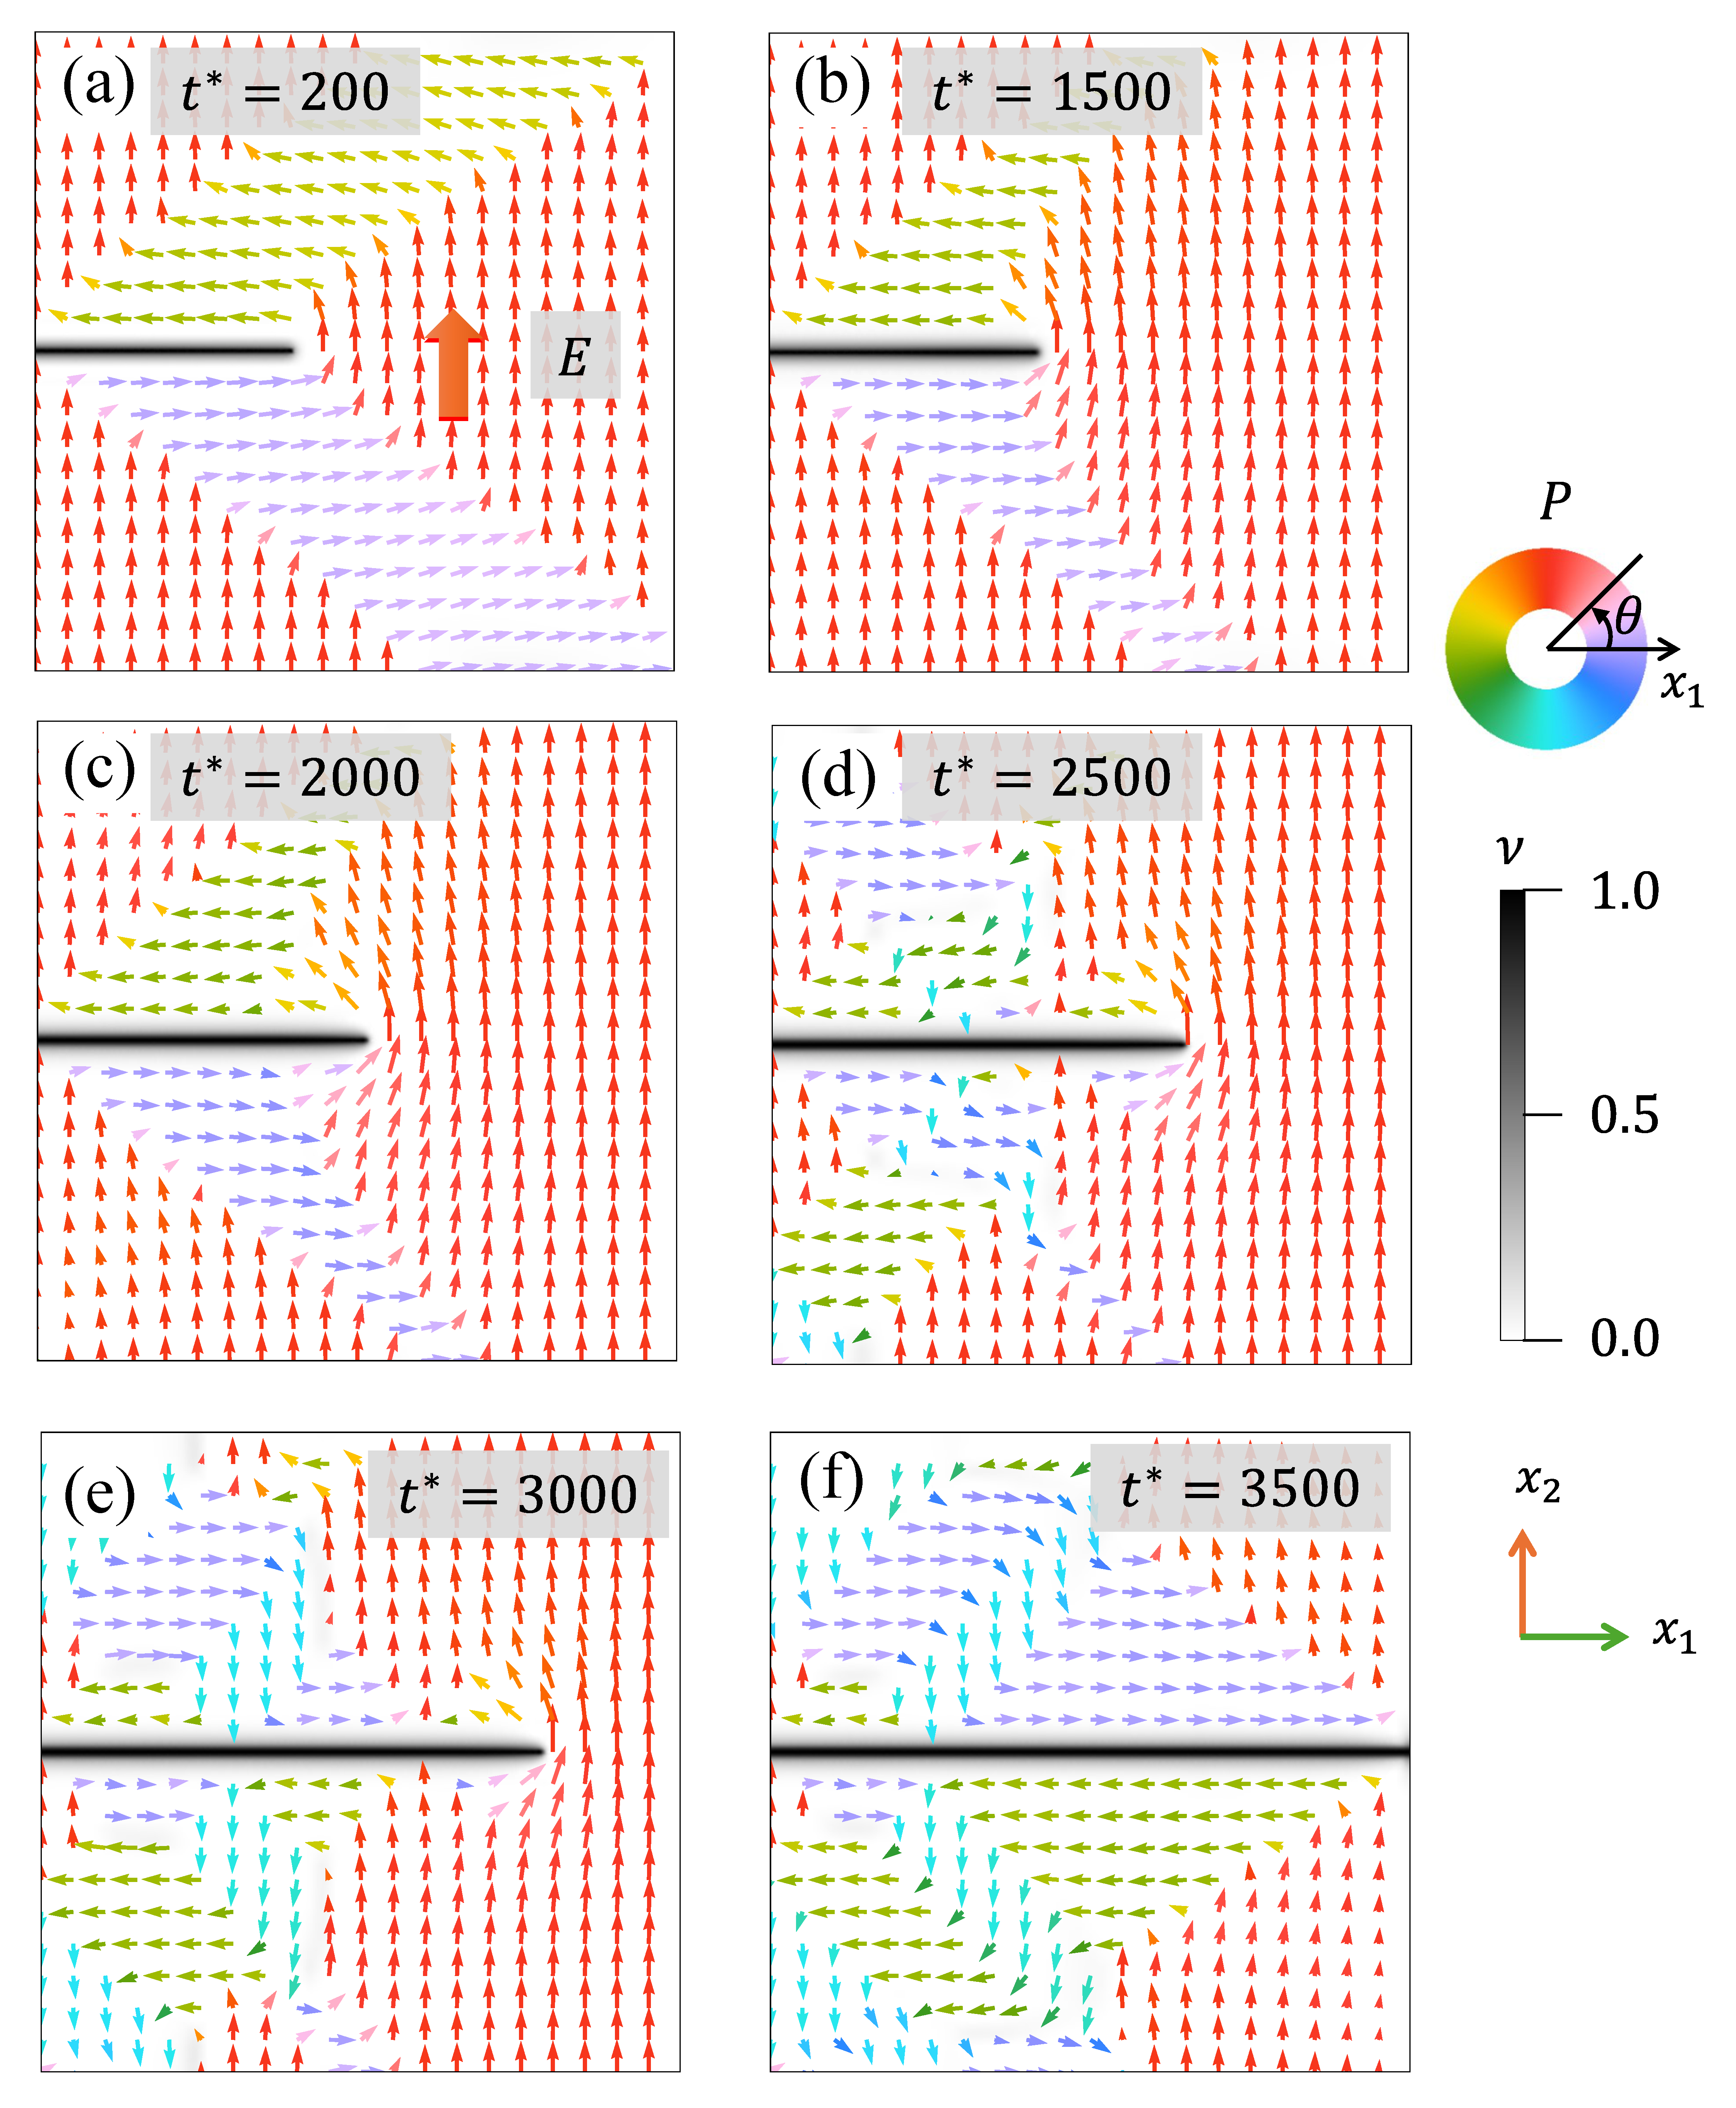
\includegraphics[width=\linewidth]{Fig10.pdf}
    \caption{Morphologies of the crack and polarization at moments $t^=200$, $t^*=1500$, $t^*=2000$, $t^*=2500$, $t^*=3000$, and $t^*=3500$ under the applied electric field $E^*_2=1$, respectively. The flexoelectric effect is neglected here.} \label{fig10}
\end{figure}

Figure \ref{fig11}(a) illustrates the evolution of crack extension $\Delta x$ over time $t$. Regardless of whether the initial polarization is along the upward or downward direction, the crack extends at the same rate. On the other hand, the crack extension is considerably postponed when the initial polarization direction is perpendicular to the crack. This delay arises due to the positive spontaneous strain $\varepsilon_{22}^0$ induced by the polarization component $P_2$, which places the plate in a compressed state under the $u_2=0$ boundary condition. Conversely, when the polarization is aligned along the $x_1$-axis, the resultant negative $\varepsilon_{22}^0$ will induce tension under the same boundary condition, thereby facilitating earlier crack extension.

The changes in the driving force $J$ and fracture toughness $J_c$ over time step $t$ are displayed in Figure \ref{fig11}(b). Similar to the results in Figure \ref{fig4}(b), $J_c$ remains stable around 20, which is close to the critical fracture toughness $G_c$. The crack begins to extend when $J$ exceeds $J_c$ at $t^*=1432$. During the period $t^*=1432$ and $t^*=2000$, $J$ exhibits a monotonic increase. During this period, the polarization-switched zone shrinks, releasing domain wall energy and accelerating the crack extension. After $t^*=2000$, corresponding to the formation of new domain walls, which consume part of the input energy. Hence, $J$ slightly decreases and slow down the crack extension. As $u_2$ continues to increase, the domain structure gradually stabilizes, and the energy input continues to rise. Consequently, $J$ begins to increase rapidly until fully fracture.

\begin{figure}[!htbp]
    \centering
    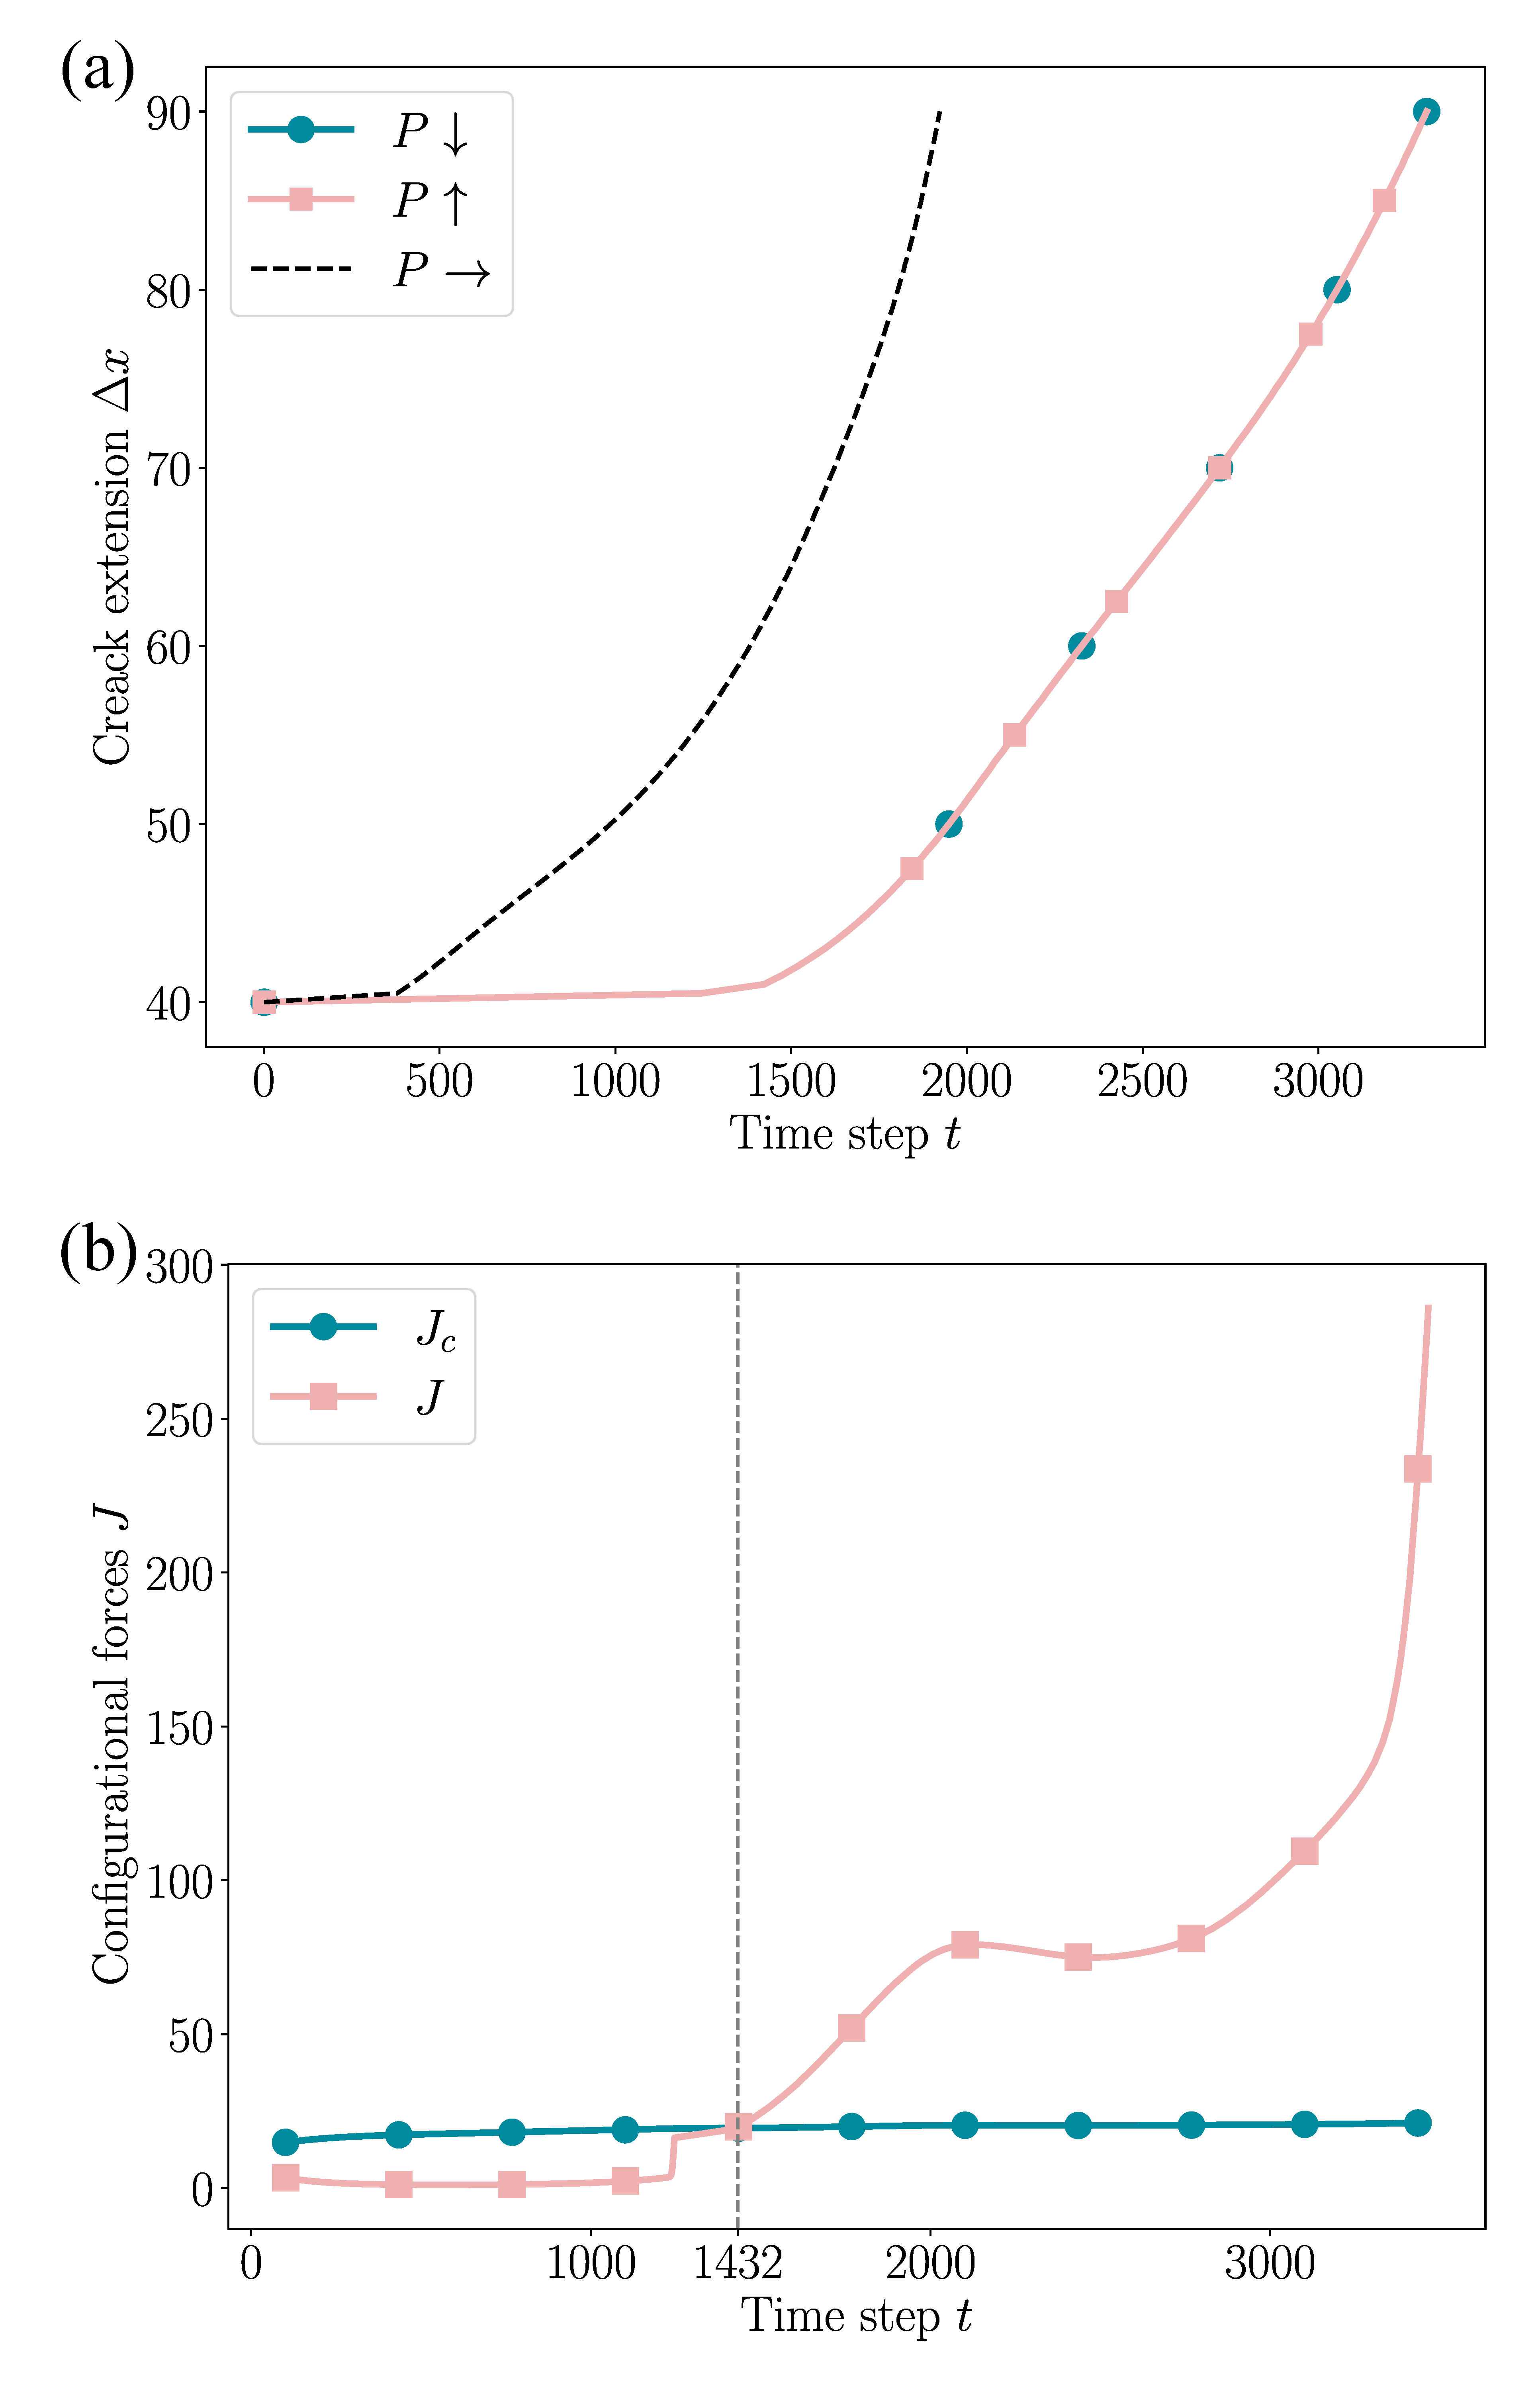
\includegraphics[width=0.7\linewidth]{Fig11.pdf}
    \caption{(a) The variation of crack extension $\Delta x$ with respect to time step $t$. The arrows in the legend denote the initial direction of polarization. (b) The change of the crack driving force $J$ and local fracture toughness $J_c$ over time step $t$. Data are collected from the cases in Figure \ref{fig9}.} \label{fig11}
\end{figure}

When the initial polarization direction is perpendicular to the crack, the flexoelectric effect also influences the crack path and the evolution of domain structures during crack propagation. Figure \ref{fig12} illustrates the temporal evolution of domain structure and crack path under an applied electric field $E_2^*=-1$, taking into account the flexoelectric effect. As shown in Figure \ref{fig12}(a), before the crack begins to extend, $90^\circ$ rotation of polarization still occur on either side of the crack, which forms two forward wings structure. However, the area of the switched zone in the upper part is significantly larger than the lower counterpart, resulting in an asymmetrical domain structure. As $u_y$ increases, the crack begins to extend and the forward wing structure disappears. With the ongoing extension of the crack, the domain structures on both sides gradually evolve into a flux-closure domain structure. Additionally, during this evolution, the domain structures on either side of the crack do not maintain symmetry, as depicted in Figures \ref{fig12}(b)-(e). After complete fracture, each side of the crack forms a complete flux-closure domain, with the upper half oriented clockwise and the lower half counterclockwise. Moreover, the flexoelectric effect induces a slight upward deflection in the crack path, which no longer remains straight. The complete spatial and temporal evolution of the domain structure and crack path is presented in Video S7.
 
\begin{figure}[!htbp]
    \centering
    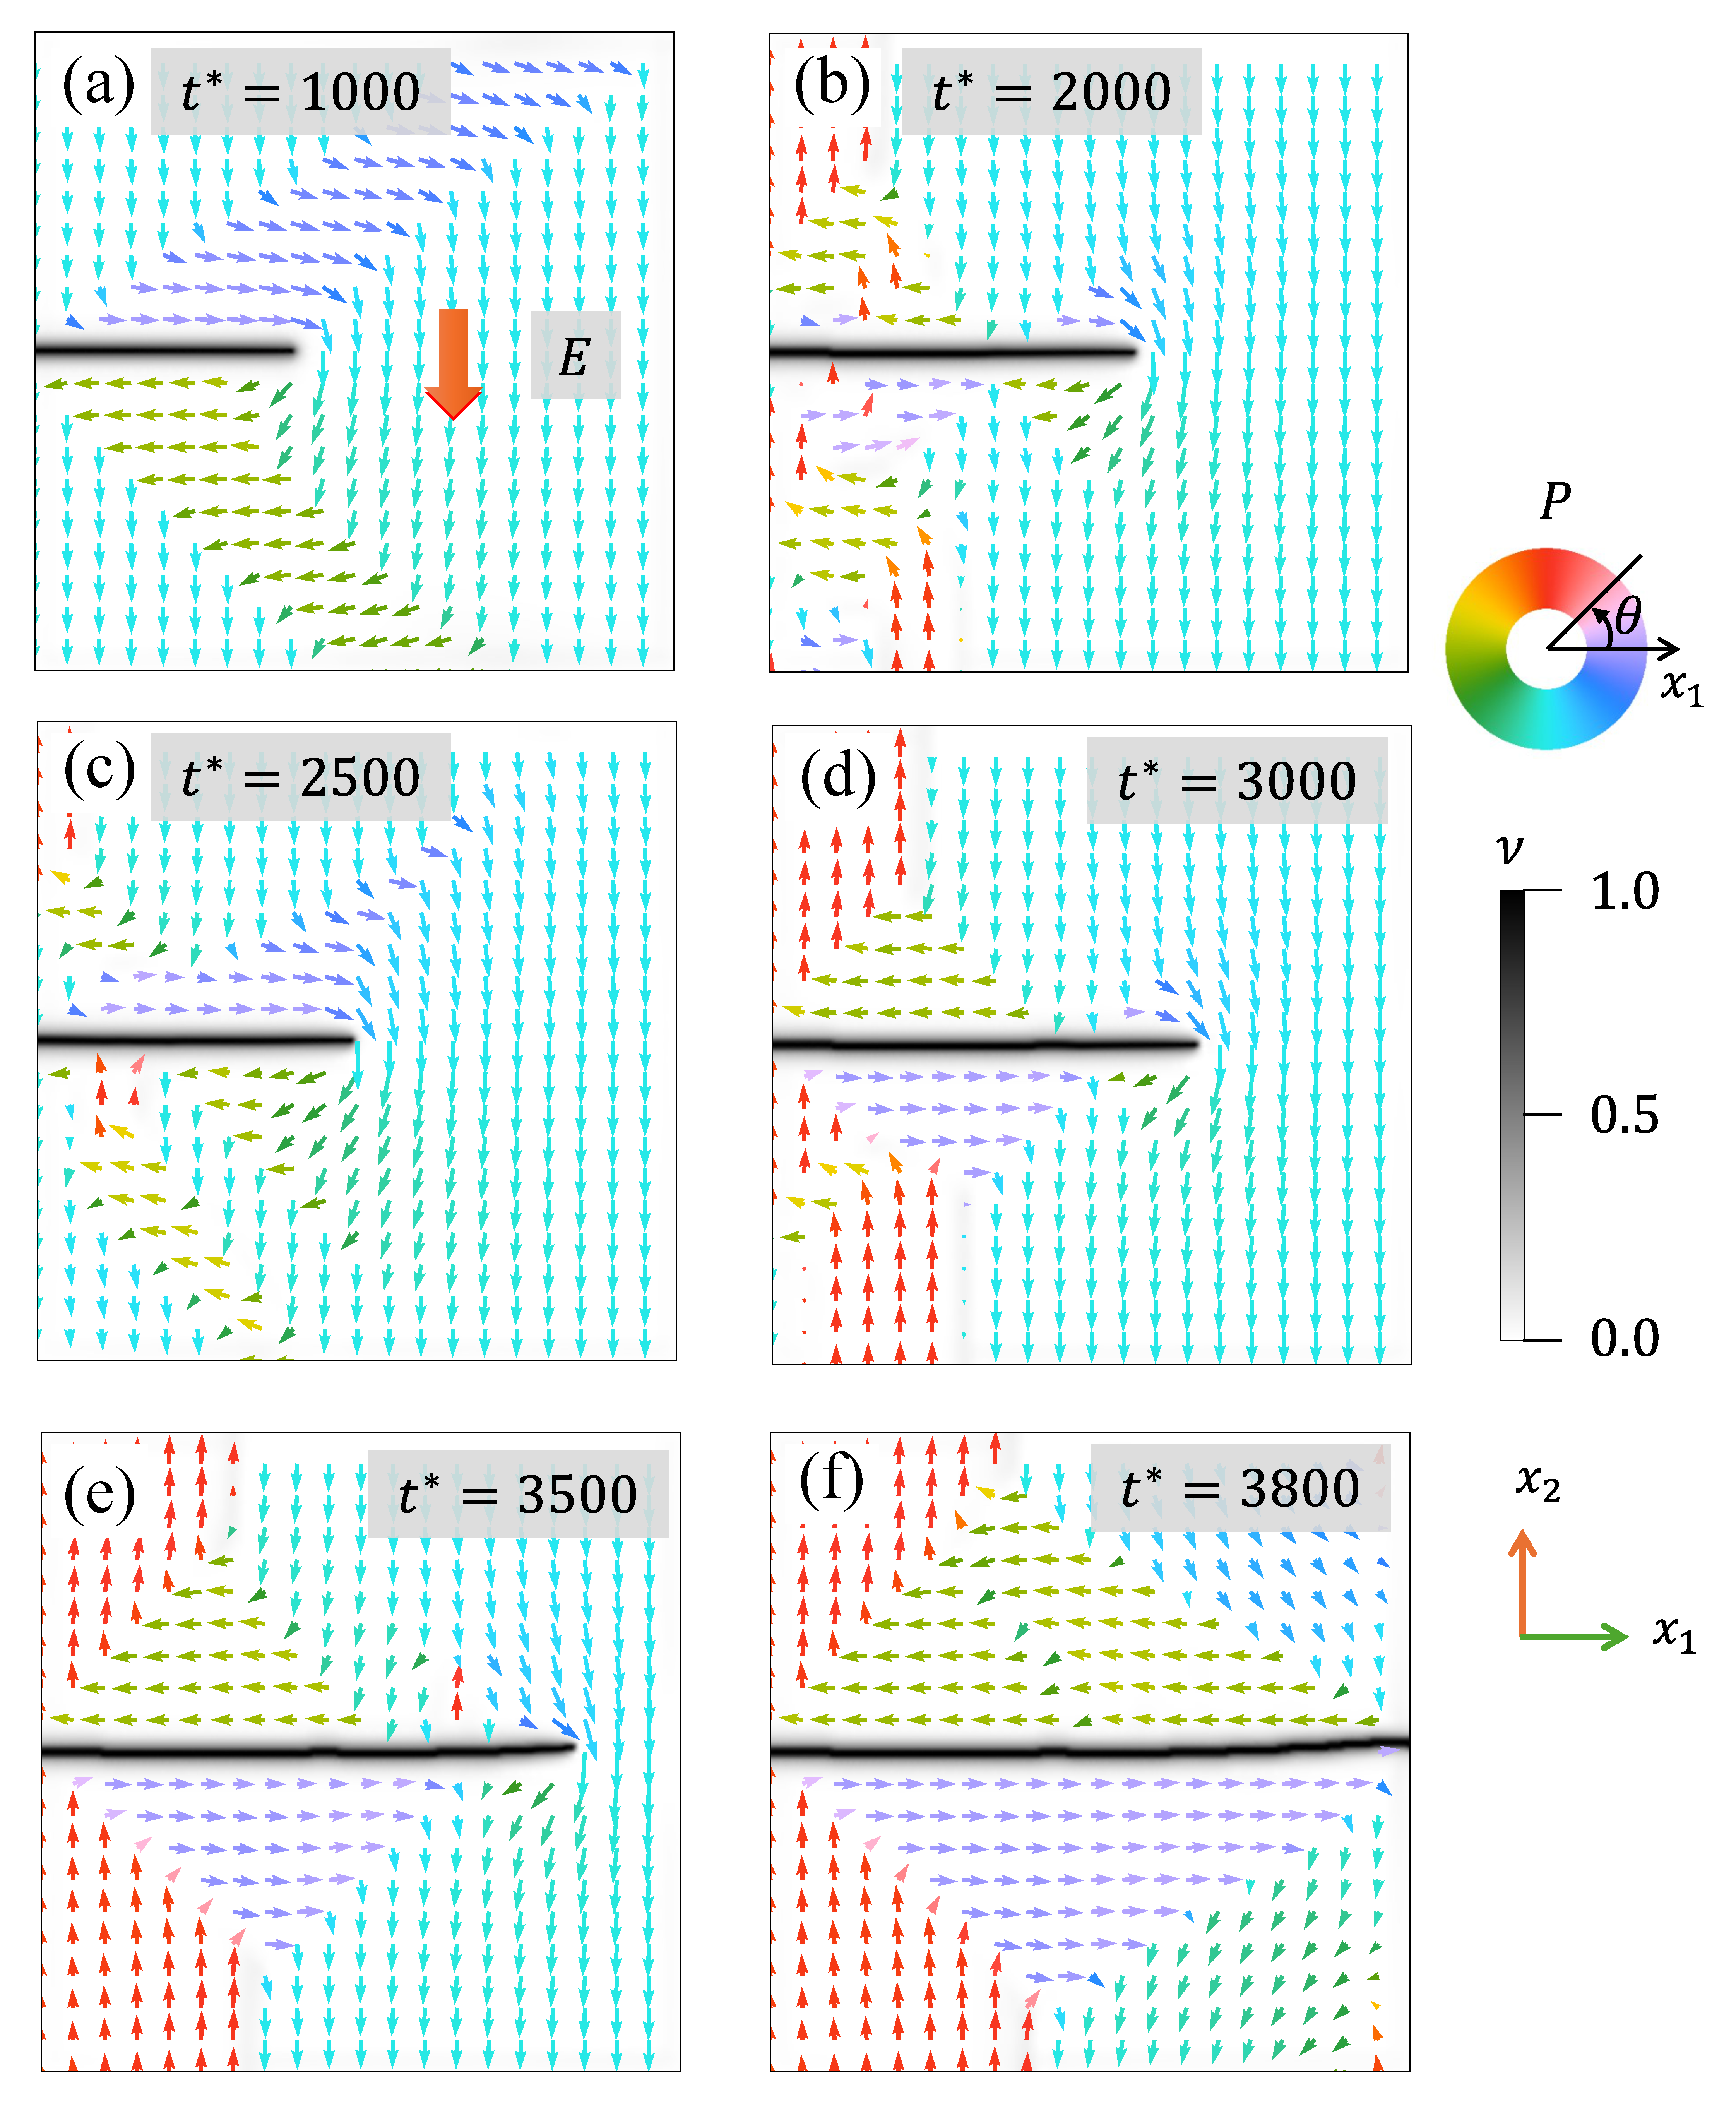
\includegraphics[width=\linewidth]{Fig12.pdf}
    \caption{With the consideration of flexoelectric effect, the evolution of polarization domain and the crack extension at moments $t^*=1000$, $t^*=2000$, $t^*=2500$, $t^*=3000$, $t^*=3500$, and $t^*=3800$ under the applied electric field $E^*_y=-1$, respectively.} \label{fig12}
\end{figure}

On the other hand, when polarization is oriented in the upward direction (applied electric field $E^*_2=1$), the temporal evolution of the crack path and domain structures over time is depicted in Figure \ref{fig13}. Compared to the results listed in Figure \ref{fig12}, the polarization direction at corresponding locations is reversed by $180^\circ$.  Additionally, the crack propagation path exhibits a downward deflection. The evolution of the domain structures and the crack extension remain consistent with those shown in Figure \ref{fig12}. Video S8 displays the complete spatial and temporal evolution of the domain structure and crack path.

\begin{figure}[!htbp]
    \centering
    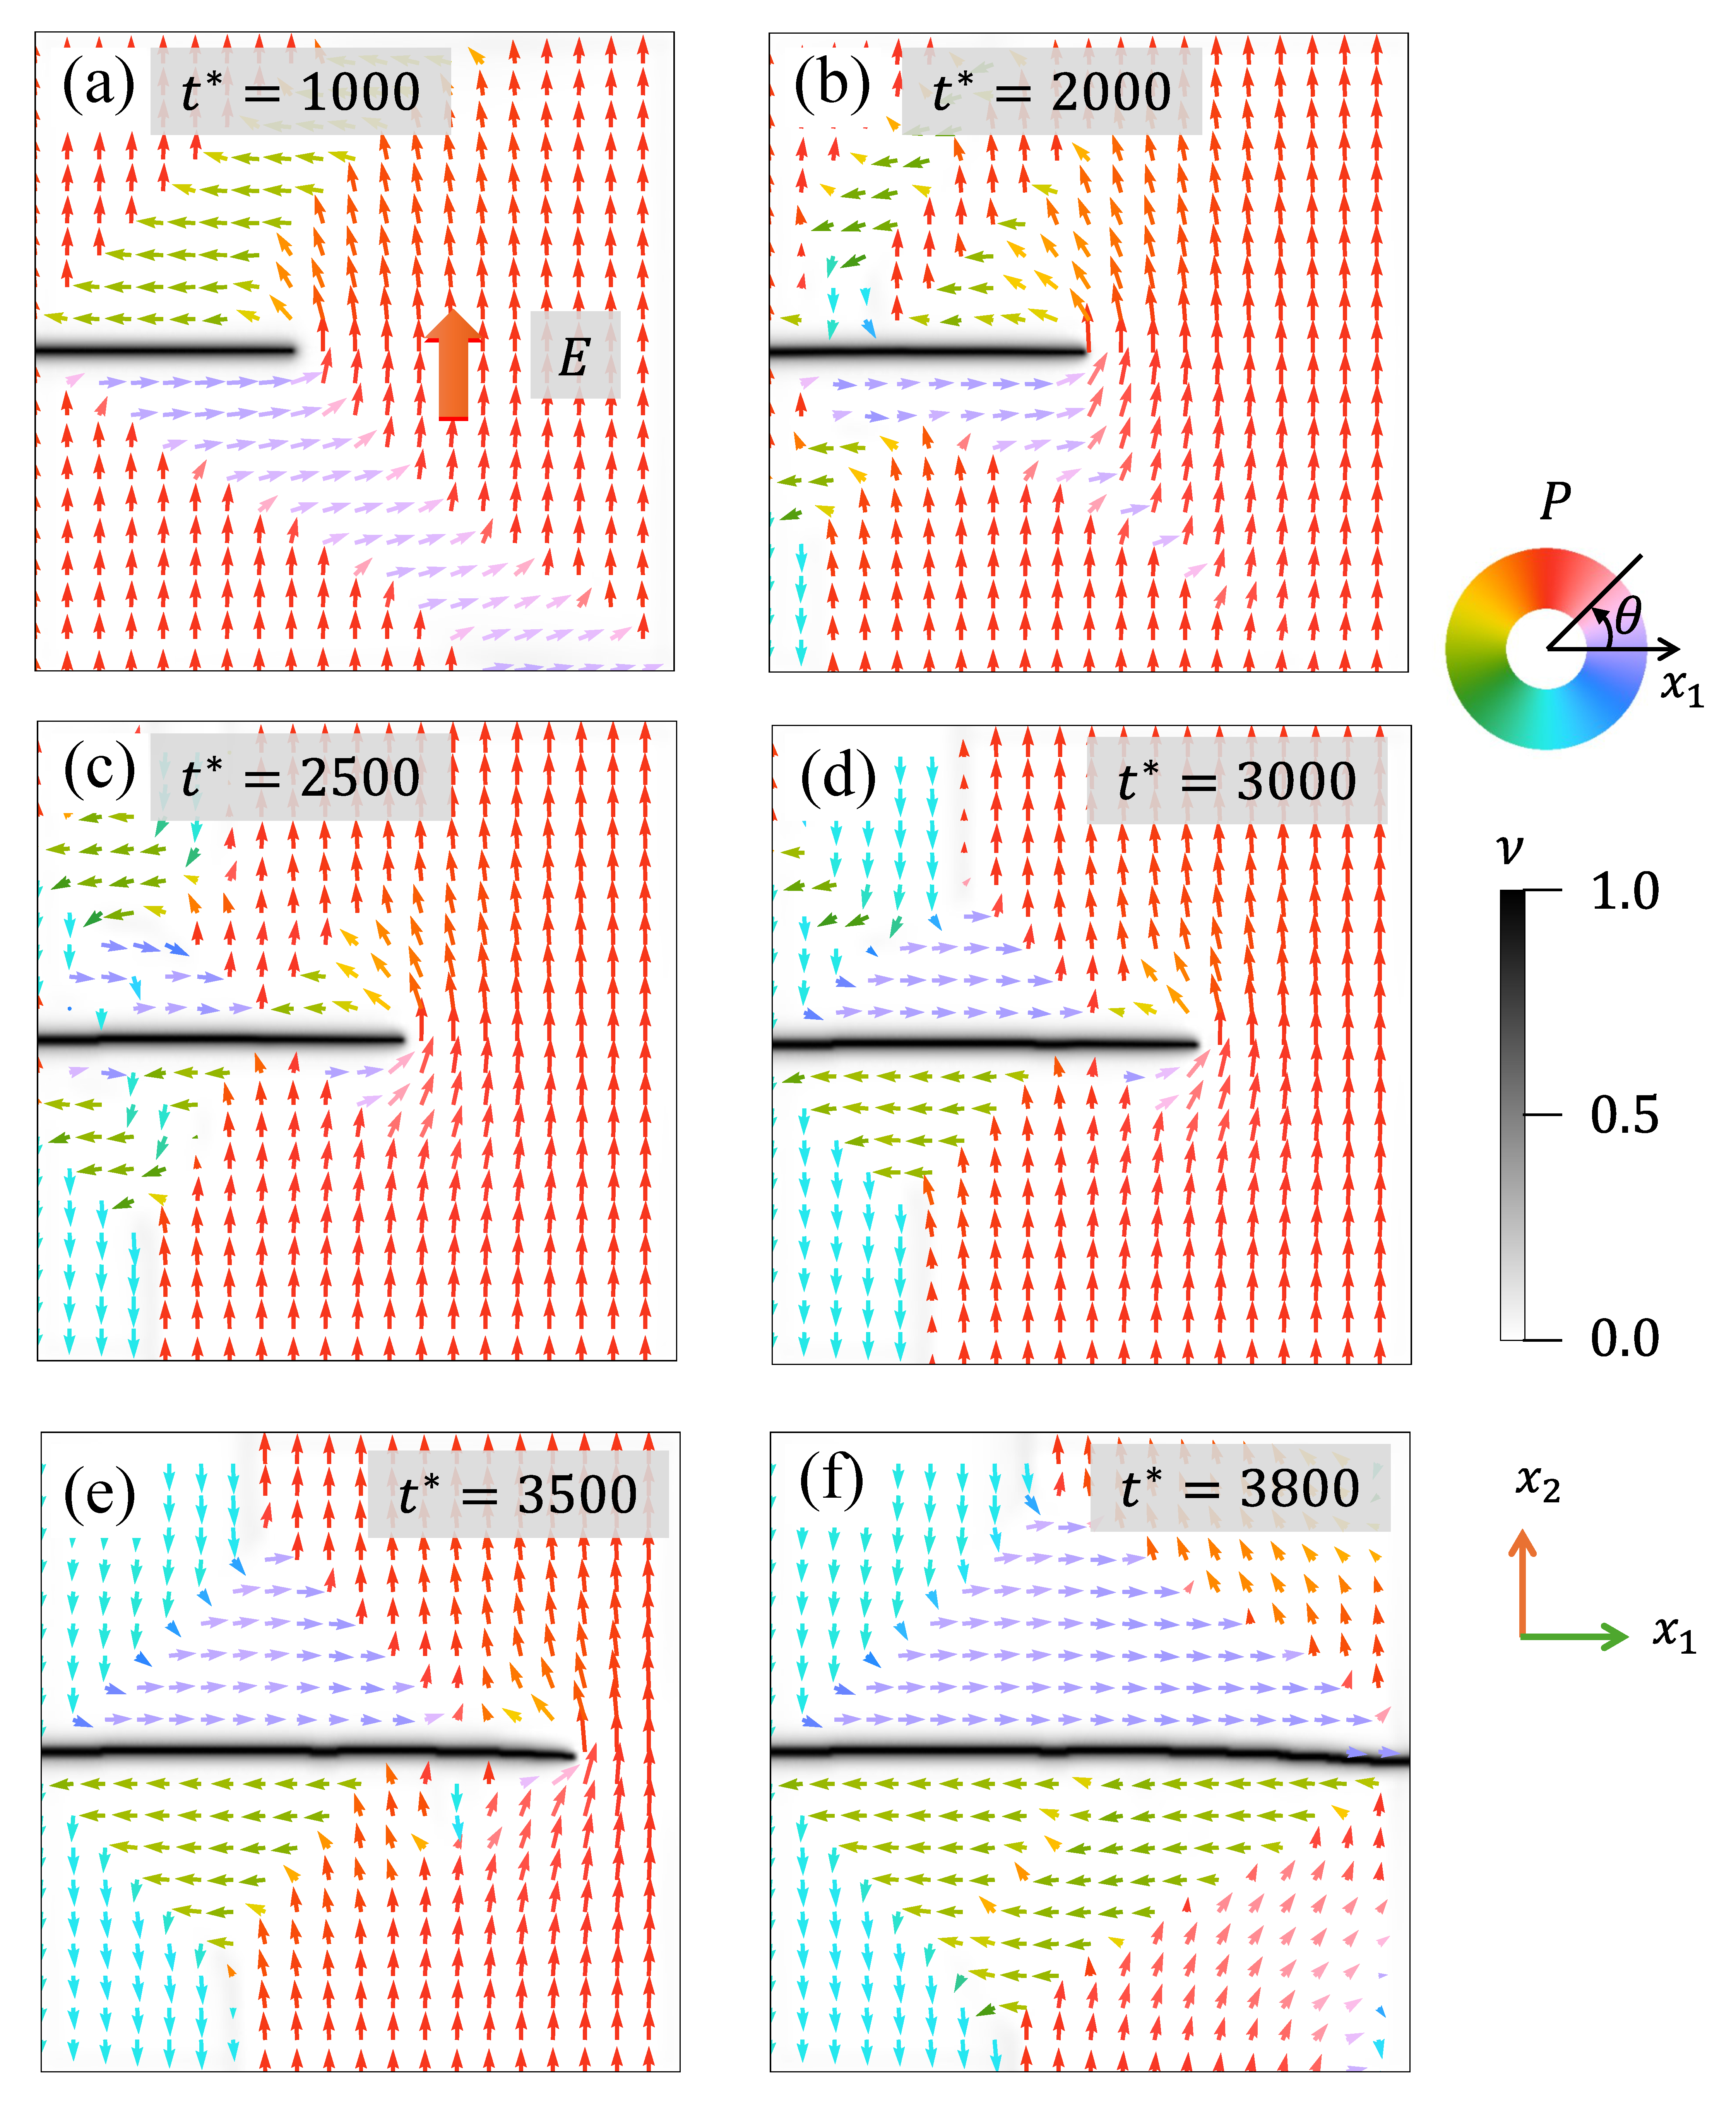
\includegraphics[width=\linewidth]{Fig13.pdf}
    \caption{Evolution of polarization domain and the crack extension at moments $t^*=1000$, $t^*=2000$, $t^*=2500$, $t^*=3000$, $t^*=3500$, and $t^*=3800$ under the applied electric field $E^*_y=1$, respectively. The flexoelectric effect is considered in this case.} \label{fig13}
\end{figure}

\begin{figure}[!htbp]
    \centering
    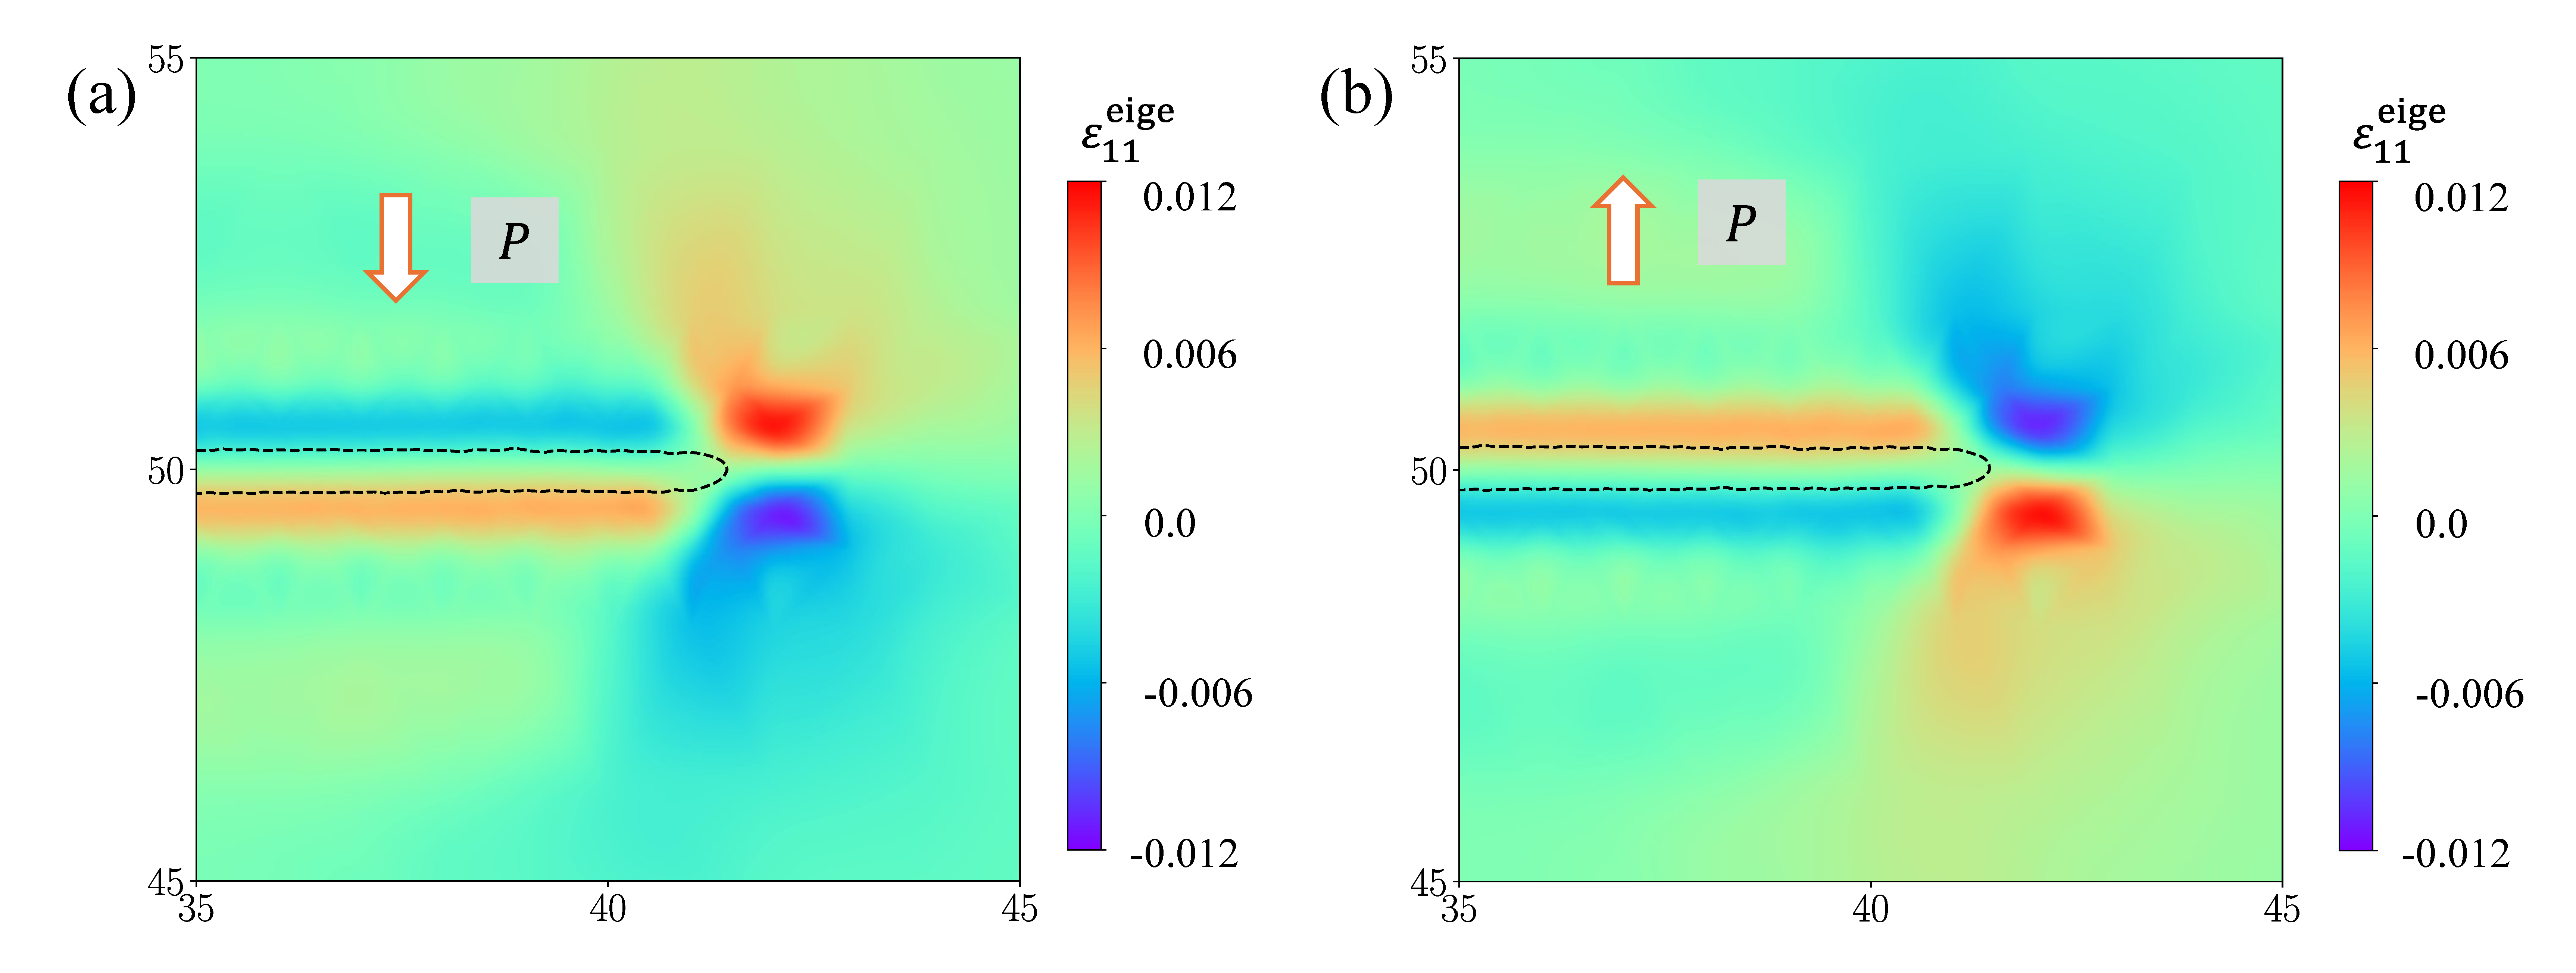
\includegraphics[width=\linewidth]{Fig14.pdf}
    \caption{Local distribution of eigenstrain $\varepsilon_{11}^{\mathrm{eige}}$ near the crack tip, for (a) initial polarization along the negative $x_2$-direction and (b) initial polarization along the positive $x_2$-direction. The dashed lines in the images mark the region of the crack ($\nu\geq0.9$)} \label{fig14}
\end{figure}

With the contribution of the flexoelectric effect, the deflection of crack path can also be attributed to the eigenstrain induced by polarization gradients. Figures \ref{fig14} show the distribution of the eigenstrain $\varepsilon_{11}^{\mathrm{eige}}$ near the crack tip at $t^*=1500$. When the initial polarization is downward, additional tensile strain develops in the upper right region of the crack tip, while the lower right region experiences additional compressive strain. Consequently, $\varepsilon_{11}^{\mathrm{eige}}$ accelerates the failure of the material in the upper right region of the crack tip, while providing shielding to the lower right region. In contrast, for the   initial polarization aligned upward, the upper right area of the crack tip experiences additional compressive strain, while additional tensile strain occurs in the lower right region. Therefore, the lower right region of the crack tip is more likely to fracture, leading to the downward deflection of the crack path.

\begin{figure}[!htbp]
    \centering
    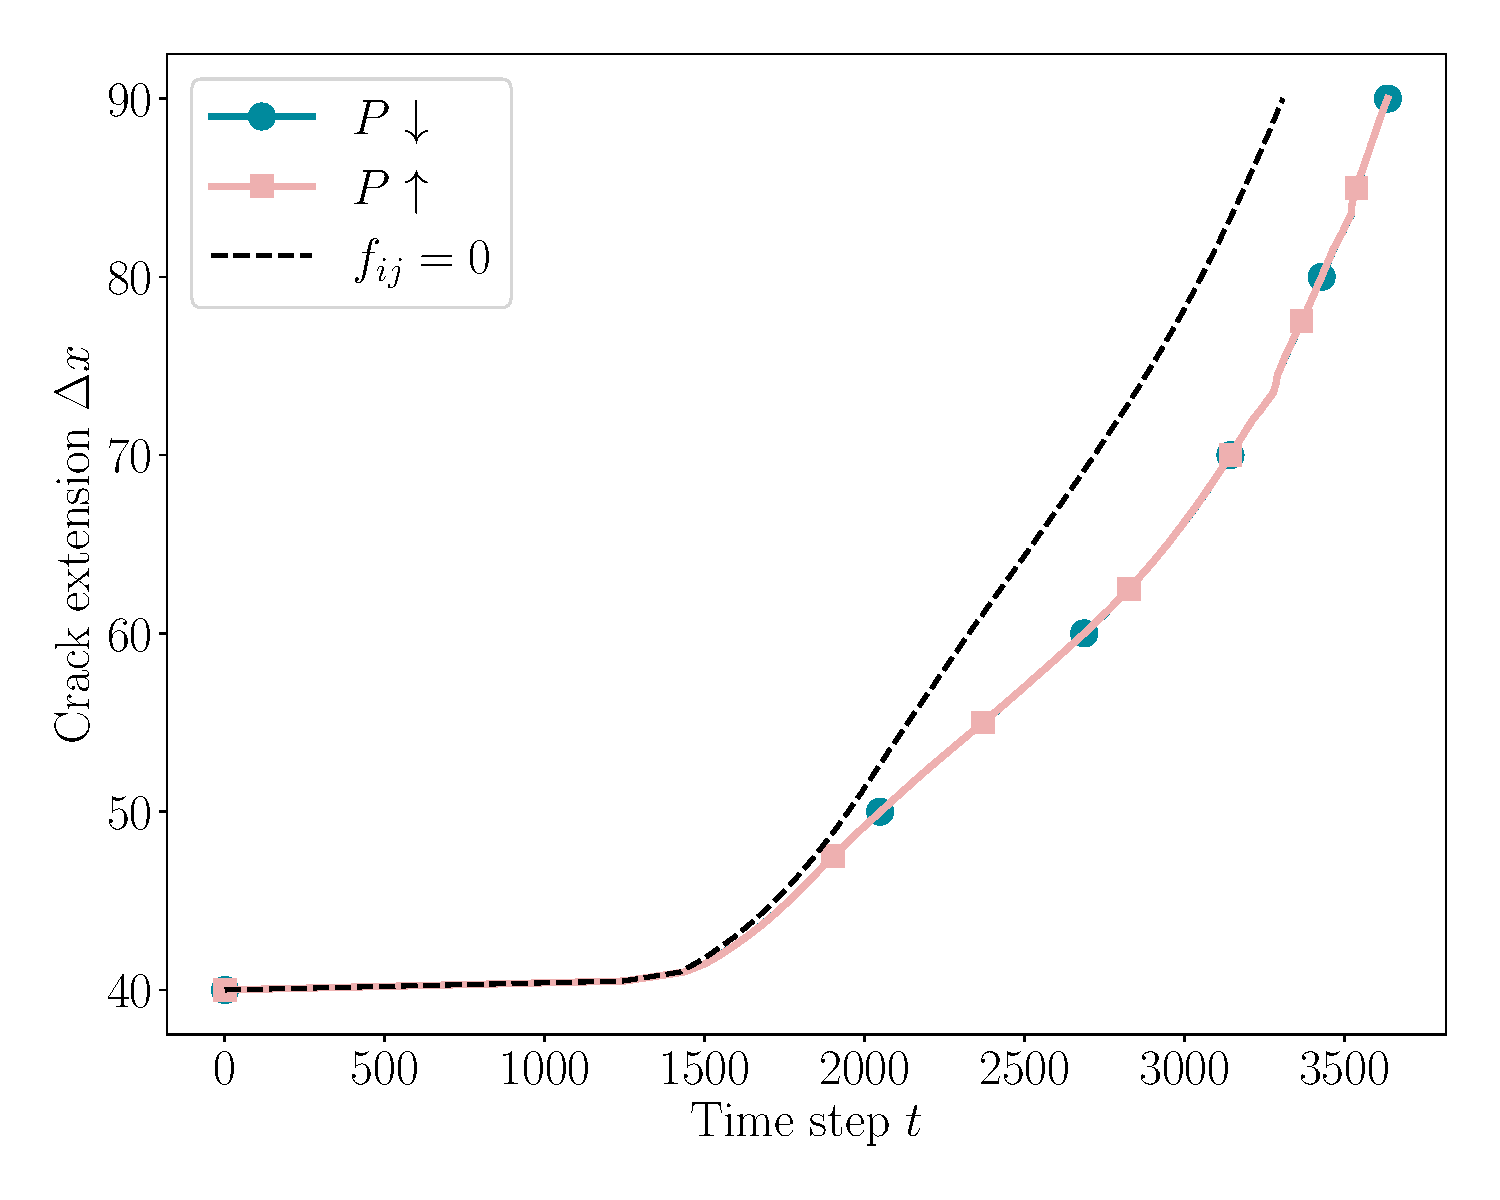
\includegraphics[width=0.7\linewidth]{Fig15.pdf}
    \caption{Crack extension $\Delta x$ over time step $t$. The solid lines represent the cases considering the flexoelectric effect, while the dashed line represents the cases without considering the flexoelectric effect. The upward and downward arrows in the legend indicate the initial polarization direction.} \label{fig15}
\end{figure}

Figure \ref{fig15} presents the crack extension $\Delta x$ over time step $t$. With the introduction of the flexoelectric effect, the onset of crack propagation is delayed. In contrast to cases where the crack is parallel to the initial polarization direction, the crack propagation rate remains identical regardless of whether the initial polarization is directed upward or downward. These simulation results are  consistent with experimental observations, which indicate that the flexoelectric effect does not alter fracture toughness when the polarization is perpendicular to the crack \cite{cordero-edwards_flexoelectric_2019}.

According to Eq.\ref{eq9}, the flexoelectric effect causes a deflection in the crack propagation path, which increases the overall crack length. Figure \ref{fig16} compares the fracture energy $\psi_\mathrm{frac}$ as a function of crack extension $\Delta x$ for cases with  or without the flexoelectric effects. Due to the presence of pre-existing cracks, the $\psi_\mathrm{frac}$ values for both cases are similar at  the initial state. As the crack extends, both cases show a monotonic increase in $\psi_\mathrm{frac}$. However, with the consideration of the flexoelectric effect, the deflection of the crack path leads to a more rapid increase in $\psi_\mathrm{frac}$, indicating that more energy is expended on crack growth.

\begin{figure}[!htbp]
    \centering
    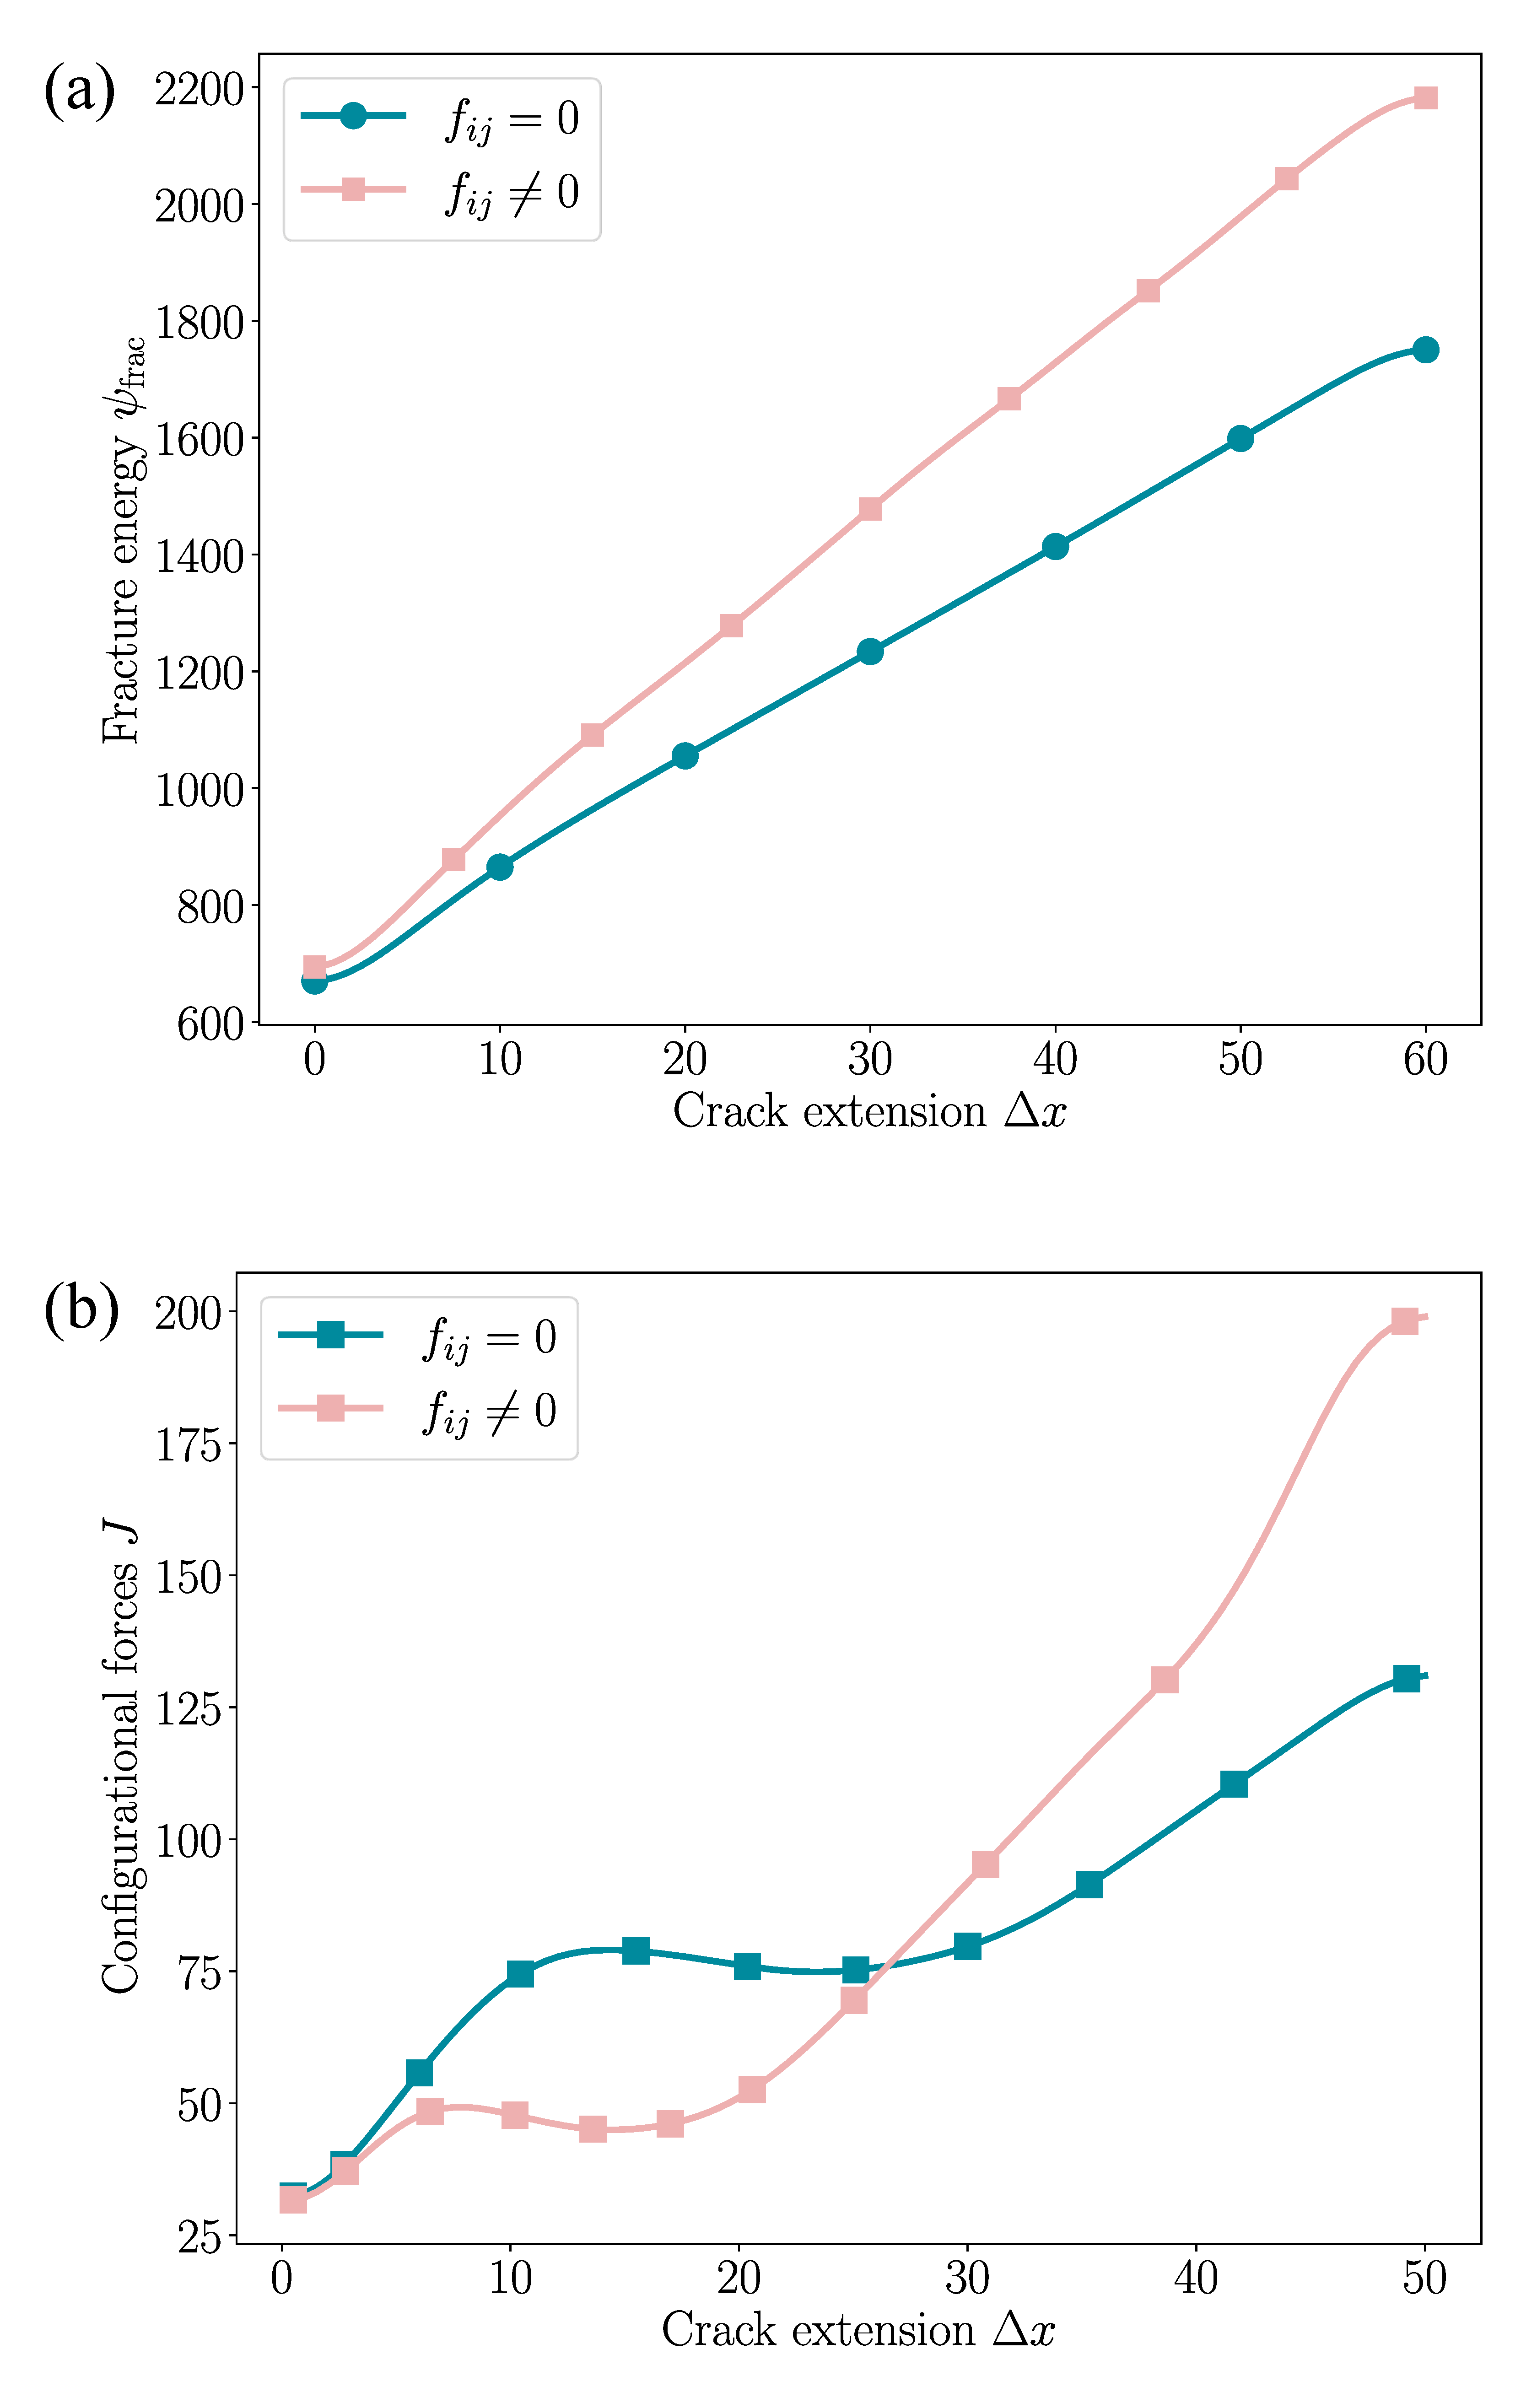
\includegraphics[width=0.7\linewidth]{Fig16.pdf}
    \caption{(a) fracture energy $\psi_\mathrm{frac}$ and (b) configurational force $J$ as functions of crack extension $\Delta x$. The data are from Figures \ref{fig9} and \ref{fig12} respectively.} \label{fig16}
\end{figure}

The difference in the fracture energy can also influence the crack driving force $J$. As presented in Figure \ref{fig16}(b), during the early stages of crack extension, the crack driving force becomes larger when the flexoelectric effect is neglected. Hence, the crack propagation rate is faster without the flexoelectric effect. This is consistent with the results that more energy is required to form a deflected crack path with the flexoelectric effect. Throughout the crack propagation, the intact region of the material is longer at the same time step compared with the case that considering the flexoelectric effect. As a result, it also stands a larger load. Consequently, as the crack extension, the difference in input energy gradually compensates for the difference in fracture energy. Therefore, in the latter stages of crack propagation with flexoelectric effect, the crack driving force is higher, and the crack extends more rapidly. 
